\documentclass{mipt-thesis-ms}
\usepackage{mipt-thesis-biblatex}
\addbibresource{bibliography.bib}
\usepackage{graphicx}
\usepackage{wrapfig}
\usepackage{hyperref}
\numberwithin{equation}{chapter}
\hypersetup{colorlinks=false}
\usepackage{float}
\usepackage{url}
%\setlength\parindent{0pt}
%\pagestyle{plain}
\usepackage{xcolor}

\newcommand{\nl}[1]{\textcolor{blue}{NL: #1}}
\begin{document}

\title{Оценка точности измерения постоянной Хаббла на основе наблюдений гравитационно линзированной сверхновой SN Refsdal}
\author{Круглов А.\ А.}
\supervisor{к.ф.-м.н. Лыскова Н.\ С.}
\referee{к.ф.-м.н. Человеков И.В.}
\groupnum{582}
%\faculty{Физтех-школа Фундаментальной и Прикладной Физики}
%\department{Кафедра космической физики}

\frontmatter
\mainmatter

%\pagenumbering{arabic}

\titlepage

\newpage
%В настоящее время значения основных космологических параметров известны с очень высокой точностью. В рамках современной стандартной космологической модели $\Lambda$CDM некоторые из них определены с точностью один процент или лучше. При этом значения постоянной Хаббла $H_0$, которая определяет темп расширения Вселенной на текущую эпоху, измеренные по ранней Вселенной, в частности, по реликтовому излучению, систематически меньше значений, измеренных по поздней Вселенной -- например, по сверхновым типа Ia и гравитационно линзированным квазарам. Эти значения не согласуются друг с другом на уровне значимости примерно $4\sigma$, что может свидетельствовать как о наличии неучтенных или неизвестных систематических эффектов, так и о новой физике, выходящей за рамки модели $\Lambda$CDM.

%Для понимания причин этого расхождения необходимо привлечение независимых подходов, способных также с высокой точностью определять фундаментальные космологические параметры. Одной из таких возможностей является использование наблюдений гравитационно линзированных систем, в частности, линзированных сверхновых. Точность оценки космологических параметров из наблюдений гравитационно линзированных систем зависит как от надежности моделирования гравитационного потенциала линзы, так и от точности определения временных запаздываний между изображениями источника. 

%При анализе гравитационно линзированных сверхновых с множественными изображениями одним из важнейших систематических эффектов является микролинзирование звездами галактики-линзы, которое может существенным образом изменять наблюдаемые кривые блеска, что в свою очередь затрудняет как моделирование кривой блеска сверхновой, так и определение временных запаздываний между изображениями, необходимые для определения космологических параметров. Как следствие, разработка алгоритма, позволяющего учесть данный эффект, является чрезвычайно актуальной и востребованной для тестирования космологической модели. 

\begin{center}
    \Large{\textbf{Аннотация}}
\end{center}

В данной работе представлен алгоритм извлечения оценки постоянной Хаббла на основе данных по всем 5 наблюдаемым изображениям сверхновой SN Refsdal (S1-S4, SX). На основе сравнения прогнозов временных задержек и коэффициентов усиления SN Refsdal, рассчитанных в различных моделях гравитационного потенциала линзы-галактики и масштабированных таким образом, чтобы они совпадали с наблюдаемыми величинами, вычислено значение постоянной Хаббла, наиболее точно удовлетворяющее и модельным, и наблюдательным данным: $H_0=68.1_{-10.0}^{+12.9}$. При анализе гравитационно линзированных сверхновых с наблюдаемыми множественными изображениями одним из важнейших систематических эффектов является микролинзирование звездами галактики-линзы, которое может существенным образом изменять наблюдаемые кривые блеска. Звезды в галактике образуют богатую сеть каустик, что приводит к тому, что наблюдаемые кривые блеска при расширении сверхновых испытывают зависящие от времени усиления/ослабления, уникальные для каждого изображения. Промоделирован вклад микролинзирования в кривые блеска SN Refsdal в модели сверхновой с реалистичным профилем яркости. Получена оценка погрешности, вносимой в определение временных задержек между изображениями S1 и S2 SN Refsdal только микролинзированием в условиях идеального эксперимента: 1-3 дня. Показано, что даже в условиях идеального эксперимента точность измерения усилений составляет порядка 1 зв.вел. 

%Работа содержит ААА страниц основного текста и БББ рисунков. При создании работы был использован ВВВ источник.
\newpage
\begin{center}
    \Large{\textbf{Благодарности}}
\end{center}

\noindent Выражаю искреннюю благодарность своему научному руководителю к.ф.-м.н. Наталье Сергеевне Лысковой за её неоценимую и профессиональную помощь при написании магистерской диссертации. За время нашей совместной работы она стала для меня образцом настоящего ученого и привила мне любовь к космической физике. Также хотелось бы поблагодарить свою семью и коллег по Школе №67, которые поддерживают меня и твёрдо уверены в моих успехах. Отдельная благодарность Петру Бакланову из ИТЭФ за научные данные, без которых было бы невозможно создание этой работы.


\newpage
\tableofcontents

\pagestyle{miptthesis}

\chapter{Введение}
В настоящее время значения основных космологических параметров известны с очень высокой точностью. В рамках современной стандартной космологической модели $\Lambda$CDM некоторые из них определены с точностью один процент или лучше. \textcolor{red}{ссылка на планк} Однако для некоторых параметров, например, для постоянной Хаббла $H_0$, определяющей  темп расширения Вселенной в современную эпоху, 
наблюдается систематическое расхождение в значениях,  измеренных по ранней и по поздней Вселенной. Так, по данным обcерватории \textit{Planck} из наблюдений реликтового излучения величина $H_0$ составляет $67.4 \pm 0.5$ км/с/Мпк (\cite{planck2018}). В то же время из наблюдений сверхновых типа Ia, так называемых «стандартных свечей», получено не зависящее от используемой космологической модели значение постоянной Хаббла, равное $74.03 \pm 1.42$ км/с/Мпк (\cite{riess2019}). \textcolor{red}{можно привести какой-нибудь график с разными методами определения H0 с указанием статьи-первоисточника, естественно.} Эти значения не согласуются друг с другом на уровне значимости примерно $4\sigma$, может свидетельствовать как о наличии неучтенных или неизвестных систематических эффектов, так и о новой физике, выходящей за рамки модели $\Lambda$CDM. Для понимания причин этого расхождения необходимо привлечение независимых подходов, способных также с высокой точностью определять фундаментальные космологические параметры, одним из которых является использование наблюдений гравитационно линзированных систем.

Гравитационное линзирование -- это отклонение  траектории света от прямолинейной в гравитационном поле массивных объектов (см., например, классические учебники по теории гравитационного линзирования \cite{schneider1992}, \cite{gravlensbook}). Важным свойством гравитационного линзирования является возможность формирования нескольких изображений одного и того же источника. Если линзированный источник является переменным, то точное измерение временной задержки между кривыми блеска, наблюдаемыми в различных изображениях, позволяет с высокой точностью оценить значение постоянной Хаббла (\cite{timedelaycosmography}),  а также других космологических параметров \textcolor{red}{(ref).}

В настоящее время в целях уточнения космологических параметров активно развиваются методы, основанные на анализе наблюдаемых гравитационно-линзированных квазаров. Многолетние наблюдения множественных изображений линзированных галактиками квазаров позволили с хорошей точностью измерить временные запаздывания между изображениями. В рамках проекта “COSMOGRAIL” (COSmological MOnitoring of GRAvitational Lenses) уже более десяти лет проводят регулярные наблюдения кривых блеска примерно тридцати линзированных квазаров и разрабатывают методы определения временных запаздываний с целью определения постоянной Хаббла с точностью ~3\%, что будет уже сравнимо с точностью, полученной из наблюдений обсерватории “Планк”. Однако в ходе выполнения данного проекта выяснилось, что проблема вырождения между гравитационным потенциалом линзы и постоянной Хаббла не позволяет достичь заявленной точности
без привлечения дополнительной информации. В связи с этим был инициирован новый проект H0LiCOW (H0 Lenses in COSMOGRAIL's Wellspring), в рамках которого для анализа были выбраны пять гравитационно-линзированных квазаров, для которых проводятся дополнительные фотометрические и спектроскопические наблюдения с высоким разрешением, в том числе измерения дисперсии скоростей звезд в галактике-линзе. Это позволит получить распределение массы с точностью до нескольких процентов и оценить постоянную Хаббла с точностью <3.5\% (Suyu et al. 2017).   
Важно отметить, что надежные измерения временных запаздываний между изображениями квазаров из наблюдений их кривых блеска требуют длительного (> 10 лет) мониторинга. Это связано с наличием как микролинзирования, так и возможной внутренней переменности квазаров на схожих с микролинзированием масштабах.
В последние годы также развивается направление исследования сверхновых, которые линзированы галактиками или скоплениями галактик. \textcolor{red}{(поправить/вставить ссылки)} Идея использования линзированных сверхновых для оценки $H_0$ была впервые предложена Сьюром Рефсдалом в 1964 году (\cite{refsdal1964}). На текущий момент известны только две гравитационно линзированные сверхновые со множественными изображениями, SN Refsdal (\cite{kelly2014}) и SN iPTF16geu (\cite{goobar2017}). Однако с запуском в ближайшее время обзора Legacy Survey of Space and Time (LSST) на обсерватории им. Веры Рубин, телескопа \textit{Roman Space Telescope}\footnote{Предыдущий вариант названия -- Wide Field Infrared Survey Telescope (WFIRST).}, а также в ходе обзора Zwicky Transient Facility на Паломарской обсерватории ожидается открытие сотен и даже тысяч таких систем \textcolor{red}{точно тысяч? Про сотни поверю, про тысячи сомневаюсь} (\cite{ogurimarshall}, \cite{goldsteinnugent2017}, \cite{veracrubin}, \cite{rst}). Наличие в обозримом будущем большого объёма наблюдательных данных делает задачу разработки алгоритма анализа гравитационно линзированных сверхновых важной и своевременной. Также предложены алгоритмы для обработки систем с неразрешёнными изображениями (\cite{beitunresolved}). 

Стоит отметить, что для сверхновых типа Ia - «стандартных свечей» - можно оценить болометрическую (интегральную по всему спектру) светимость из независимых от линзирования соображений, а значит, получить абсолютное значение усиления светового потока. Эта информация, недоступная для линзированных квазаров, позволяет уменьшить количество свободных параметров модели линзы и снять определенные вырождения (\cite{falco1985}, \cite{holz2001}, \cite{ogurikawano2003}), а значит, уменьшить ошибки на  оцениваемые космологические параметры. Кроме того, по результатам наблюдений гравитационно линзированных сверхновых типа Ia можно уточнить шкалу расстояний в астрономии (\cite{ddr}).

Гравитационно линзированные сверхновые важны не только для космологии, но и открывают новые возможности для изучения физики сверхновых, в частности, их звёзд-предшественников. \nl{В принципе, в линзированных сверхновых со множественными изображениями возможно наблюдение момента взрыва сверхновой,} %такие системы позволяют наблюдать взрыв сверхновой с самого начала, 
что ранее не представлялось возможным, учитывая сложность обнаружения сверхновых на ранних фазах и необходимость организации последующих наблюдений. Используя временную задержку между появлением различными изображениями, можно смоделировать линзирующую систему и на основе первого изображения (или нескольких изображений) сверхновой предсказать \nl{и пронаблюдать} появление следующих изображений. Наблюдения на ранней фазе имеют решающее значение для понимания природы предсверхновых (\cite{holismokesI}).

Как уже было сказано выше, в обозримом будущем ожидается обнаружение большого количества линзированных сверхновых с разрешенными изображениями.  Следует отметить,  что точность оценки космологических параметров из наблюдений гравитационно линзированных систем зависит как от надежности моделирования гравитационного потенциала линзы, так и от точности определения временных запаздываний между изображениями источника. Поэтому новой и чрезвычайно актуальной становится задача учета и минимизации возможных систематических эффектов, которые способны существенным образом изменять кривые блеска сверхновых и влиять на точность определения космологических параметров. Одним из таких эффектов является микролинзирование - гравитацинное линзирование на отдельных звёздах в галактике-линзе, уникальное для каждого изображения источника.  

Большое количество публикаций посвящено влиянию микролинзирования на кривые блеска гравитационно линзированных квазаров (одна из первых работ: \cite{changrefsdal1979}), рассмотрена зависимость значимости этого эффекта в зависимости от размера и профиля яркости квазара (\cite{sizeiseverything}), разработаны программы для численного моделирования микролинзирования квазаров (\cite{wambsganss1992}). Однако переменность их блеска непредсказуема, и для точных измерений временных задержек между изображениями необходимо накопить многолетний массив данных. \nl{Согласно оценкам, приведенным в работе \cite{20years}, для компенсации ошибок, вызванных влиянием микролинзирования на кривые блеска гравитационно линзированных квазаров, необходимо проводить наблюдения в течение 20 лет.} \textcolor{green}{Кроме того, в некоторых случаях вариации блеска
квазаров \texbf{по амплитуде?? По времени??} сопоставимы с масштабом флуктуаций, вносимых микролинзированием} (источник).

В отличие от квазаров, кривые блеска сверхновых имеют чётко выраженный пик, а их наблюдения занимают сравнительно небольшие времена, что значительно упрощает измерения временных задержек между изображениями и, как следствие, постоянной Хаббла. \textcolor{green}{Также в случае со сверхновыми проще промоделировать галактику-линзу, так как квазары могут быть очень яркими и "засвечивать" элементы гравитационно линзированной системы. Сверхновые не менее яркие, но они постепенно тускнеют и позже позволяют чётко увидеть родительскую галактику и галактику-линзу.} Тем не менее, микролинзирование может вносить существенные искажения в форму кривых блеска гравитационно линзированных сверхновых (\cite{doblerkeeton2006}). Методика минимизации влияния микролинзирования на ошибки временных задержек предложена только для сверхновых типа Ia (\cite{moresuyu2017}, \cite{goldstein2018}, \cite{foxleymarrable2018}, \cite{bonvin2019}, HOLISMOKES-III: \cite{holismokesIII}). В упомянутых работах, помимо прочего, показано, что микролинзирование на ранних стадиях расширения сверхновой может быть хроматичным, то есть зависящим от длины волны, тогда как в целом гравитационное линзирование ахроматично. Кроме того, кривые блеска сверхновых типа Ia поддаются стандартизации (\cite{1a_standart}). Однако для сверхновых с коллапсирующим ядром, к которым относится SN Refsdal (\cite{kelly2016}), необходимо разработать новые алгоритмы (HOLISMOKES-V: \cite{holismokesV}), так как их кривые блеска демонстрируют большое разнообразие, что не позволяет их использовать как стандартные свечи напрямую. В преддверии грядущих обзоров, активно  разрабатывается  программное обеспечение для анализа и моделирования наблюдений линзированных сверхновых (\cite{pierelrodney2019}), а также ведется работа по определению наиболее оптимальной тактики проведения наблюдений (\cite{hubersuyu2019}). Детальное моделирование кривых блеска сверхновых II типа может дать ценную информацию не только о строении предсверхновых, в том числе находящихся на больших красных смещениях, но и обеспечить высокую точность измерения временных задержек и определения коэффициента усиления изображений сверхновой в отсутствие микролинзирования.


SN Refsdal - первая обнаруженная линзированная сверхновая со множественными изображениями и измеренными кривыми блеска для каждого изображения - открывает эру практического использования линзированных сверхновых для тестов космологических моделей (\cite{grillo2018}). Более того, её наблюдения предоставили возможность определить физические параметры предсверхновой и детально промоделировать кривые блеска столь удаленной сверхновой ($z = 1.5$), что было бы невозможно в отсутствии линзы. На данный момент опубликованы кривые блеска первой гравитационно-линзированной сверхновой с коллапсирующим ядром SN Refsdal, для которой наблюдались пять ее изображений (\cite{rodney2016}). На основе этих данных проведено детальное моделирование кривых блеска, оценены параметры предсверхновой, уточнены временные запаздывания между изображениями и определены относительные коэффициенты усилений (\cite{petrnat2020}). 

(?) Это в том числе позволяет провести сравнение возможных моделей распределения вещества в скоплении галактик MACS J1149+2223, выступающего в роли линзы. Так как помимо микролинзирования, другим источником возможных систематических ошибок является используемая модель линзы, для уточнения которой необходимо привлекать дополнительные данные, например, оптические измерения дисперсии лучевых скоростей. Для оценки надежности методов определения гравитационного потенциала скоплений на основе оптических данных необходимы большие выборки скоплений галактик, которые стали доступны только в последнее время, что также определяет новизну и новые пути решения поставленной задачи.

\textcolor{green}{Отдельный интерес представляют системы, в которых учитывается протяженность источника и распределение его поверхностной яркости. Учёт этих особенностей может наложить дополнительные ограничения на линзирующий потенциал.Однако в этом случае требуется одновременное определение поверхностной яркости источника и потенциала линзы (\cite{suyu2010}).}

\chapter{Гравитационное линзирование}

\section{Общие сведения}
%\subsection{Гравитационно-линзированная система}

\nl{Лучше начать как-нибудь по-другому, чтобы диплом читался как единый текст. В духе: Гравитационное линзирование - это ... Выделяют два режима  - сильный и слабый. Описание. Здесь и далее речь пойдет об эффекте сильного линзирования. } В этом разделе приведены основные понятия, связанные с описанием так называемого \textit{сильного} гравитационного линзирования. Большая часть информации в данном разделе подробно представлена в книге  (\cite{gravlensbook}). В рамках общей теории относительности можно показать, что в гравитационном поле точечного массивного тела \textit{(линзы)} с ньютоновским потенциалом $\Phi$ угол отклонения светового луча равен

\begin{equation}
\hat{\alpha}=\frac{2}{c^{2}} \int_{-\infty}^{+\infty} \vec{\nabla}_{\perp} \Phi \ \mathrm{d} z,
\end{equation}

где $z$ - координата вдоль невозмущённой траектории распространения света (\cite{gl_all}). При этом предполагается, что $\Phi/c^2 \ll 1$, что выполняется практически всегда: например, для самых массивно гравитационно связанных объектов во Вселенной -- скоплений галактик --  $|\Phi|/c^2 \sim 10^{-4} \ll 1$. Это же условие обеспечивает малость углов: при сильном линзировании углы отклонения света порядка угловых секунд. Из того, что $\Phi$ не зависит от массы тела, попавшего в гравитационное поле, следует, что все фотоны отклоняются на один и тот же угол. Таким образом, сильное гравитационное линзирование ахроматично, то есть не зависит от длины волны. 
%Для точечной линзы $\Phi=-\frac{G M}{r}$, где $M$ - её масса, а значит, что углы отклонения массивом таких линз могут быть сложены по принципу суперпозиции. 

Непосредственно преломление происходит на очень коротком участке траетории света. В реалистичных моделях линз, в которых масса, вызывающая линзирование, распределена трёхмерным образом, используется приближение плоских линз по аналогии с геометрической оптикой. Это всегда оправдано: характерные размеры самого большого объекта, который может быть линзой, - скопления галактик - порядка 1 Мпк, в то время как продольные расстояния между объектами системы порядка 100-1000 Мпк. Типичная гравитационно-линзированная система изображена на Рисунке \ref{fig:gravlensfig}. Углами $\boldsymbol{\beta}$ и $\boldsymbol{\theta}$ задаются положения источника света и его изображения соответственно. Угол отклонения светового луча $\alpha$ по порядку величины составляет 1 угловую секунду при сильном линзировании на галактике.

\begin{figure}[H]
    \centering
	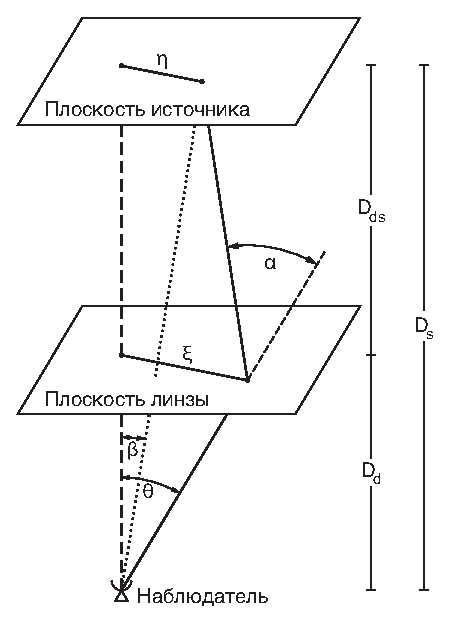
\includegraphics[scale=1.0]{pics/Gravitational_Lensing_Strong_Weak_and_Micro.eps}
	\caption{Типичная гравитационно линзированная система (\cite{gravlensbook}). Здесь $\beta$ и $\theta$ - углы между оптической осью (пунктирная линия) и источником и его изображением соответственно, $\alpha$ - угол отклонения светового луча, $\eta$ и $\xi$ - расстояния от оптической оси до источника и его изображения соответственно,  $D_d$ - расстояние между наблюдателем и плоскостью линзы, $D_{ds}$ - между плоскостями линзы и источника, $D_s$ - между наблюдателем и источником. Следует отметить, что в общем случае, $D_s \neq D_d + D_{ds}$. \label{fig:gravlensfig} }
   \end{figure} 
Уравнение линзы (соотношение между положениями источника, его изображения и углом преломления): - ПРОВЕРИТЬ

\begin{equation}\label{nablapsi}
\boldsymbol{\beta} = \boldsymbol{\theta} -  \hat{\alpha}(\boldsymbol{\theta}), \textrm{где} \  \hat{\alpha}(\boldsymbol{\theta}) = \frac{D_S}{D_{DS}}\nabla \boldsymbol{\theta}
\end{equation}



Можно показать, что

\begin{equation}\label{nabla2psi}
\kappa({\boldsymbol{\theta}}) = \frac{1}{2}\nabla^2 \Psi(\boldsymbol{\theta}),
\end{equation}

где $\kappa$  - безразмерная поверхностная плотность масс в линзе  (\textit{convergence}), $\Psi(\boldsymbol{\theta})$ - линзирующий гравитационный потенциал. Пусть масса линзы распределена в пространстве по закону $\rho(D_d \boldsymbol{\theta}, z)$, где $z$ - координата вдоль оптической оси. \textit{Поверхностная плотность} линзы задаётся следующим соотношением:

\begin{equation}\label{sigmasurf}
\Sigma(D_d \boldsymbol{\theta})=\int \rho(D_d \boldsymbol{\theta}, z) \mathrm{d} z
\end{equation}

С учётом этого для $\kappa$ также верно соотношение

\begin{equation}\label{convergence}
\kappa = \frac{\Sigma(D_d \boldsymbol{\theta})}{\Sigma_{crit}}, \ \ \ \ \  \textrm{где} \ \ \ \ \ \ \Sigma_{crit}=\frac{c^{2}}{4 \pi G} \frac{D_{\mathrm{s}}}{D_{\mathrm{d}} D_{\mathrm{ds}}},
\end{equation}

($c$ - скорость света, $G$ - гравитационная постоянная, $D_d$, $D_s$ и $D_{ds}$ - расстояния от наблюдателя до плоскости линзы, до источника и между плоскостями линзы и источника соответственно (см. Рис. \ref{fig:gravlensfig}).) По порядку величины $\Sigma_{crit} \sim 1 \ \textrm{г/см}^2$. Радиус такой окружности в плоскости линзы, плотность внутри которой равна критической ($\kappa =  1$), называется \textit{радиусом Эйнштейна}. Обычно он выражается в угловых единицах: 

\begin{equation}\label{r_ein}
\theta_{E}=\sqrt{\frac{4 G M}{c^{2}} \frac{D_{d s}}{D_{d} D_{s}}},
\end{equation}
где $M$ - масса линзы. Эта величина характеризует масштабы гравитационного линзирования и является основной шкалой расстояний при описании этого явления.

%\subsection{Усиление и искажение изображений}

В терминах линейной алгебры, гравитационное линзирование - это отображение плоскости источника на плоскость линзы, которое задаётся следующей матрицей:

\begin{equation}
\mathcal{A}(\boldsymbol{\theta})=\frac{\partial \boldsymbol{\beta}}{\partial \boldsymbol{\theta}}=\left(\delta_{i j}-\frac{\partial^{2} \psi(\boldsymbol{\theta})}{\partial \theta_{i} \partial \theta_{j}}\right)=\left(\begin{array}{cc}{1-\kappa-\gamma_{1}} & {-\gamma_{2}} \\ {-\gamma_{2}} & {1-\kappa+\gamma_{1}}\end{array}\right)
\end{equation}

Безразмерная плотность  $\kappa$ \textit{(convergence)}  отвечает за изотропное изменение линейных размеров изображения (увеличение или уменьшение),  двухкомпонентный сдвиг \textit{(shear)} $\gamma=(\gamma_1,\gamma_2)$, характеризует анизотропное искажение формы изображений. \textcolor{green}{КАРТИНКУ} Усиление изображения обратно пропорционально определителю этой матрицы (то есть якобиану этого отображения):

\begin{equation}
\mu=\frac{1}{\operatorname{det} \mathcal{A}} =  \frac{1}{(1-\kappa)^2-|\gamma|^2}
\end{equation}

Возможно существование некоторого множества точек, для которых выполняется соотношение $\operatorname{det} \mathcal{A}=0$, в которых усиление формально бесконечно \nl{добавить footnote, что в реальности бесконечных усилений не наблюдается, так как...}. Кривая, образуемая этими точками, называется каустикой, а её образ в плоскости линзы – критической кривой. 



%На Рисунке \ref{fig:caustics} видно, как ведёт себя изображение компактного источника при пересечении им складки \textit{(fold)} или излома \textit{(cusp)} каустики.
 
%\begin{figure}[H]
%    \centering
%	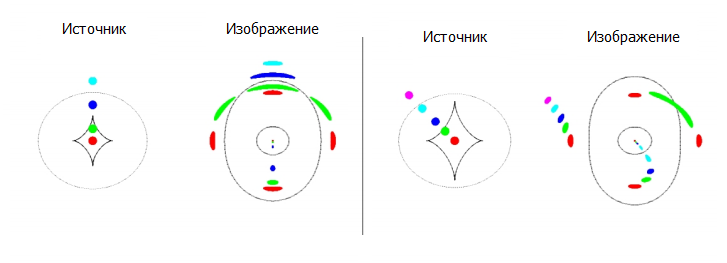
\includegraphics[scale=0.8]{pics/caust_intro.png}
%	\caption{Поведение изображения компактного источника при пересечении им излома (левая панель) или складки (правая панель) каустики  (\cite{narbart}). Также для иллюстрации изменения масштабов изображения нарисованы критические кривые в плоскости линзы. \label{fig:caustics}}
%\end{figure}



\section{Формирование нескольких изображений}
\nl{В космологии есть несколько способов определения расстояний (Hogg1999).  }
%Здесь и далее 
Для описания расстояний между объектами в системе источник - линза - наблюдатель используется понятие расстояния углового диаметра (\textit{angular diameter distance}). Оно определяется следующим образом:
%(\cite{distance_measures}, в данной публикации приведены и другие способы определения расстояния, используемые в космологии):

\begin{equation}\label{ang_dia_dist}
D_{A}\left(z_{1}, z_{2}\right)=\frac{c}{1+z_{2}} \int_{z_{1}}^{z_{2}} \frac{d z}{H_{0} \sqrt{\Omega_{m}\left(1+z\right)^{3}+\Omega_{\Lambda}}},
\end{equation}
где $z_1, z_2$ - красные смещения  соответственно линзы и источника. В данной работе мы рассматриваем плоскую Вселенную со следующими параметрами: $H_0=70$ (км/с)/Мпк, $\Omega_m=0.3, \Omega_\Lambda=0.7$.
%Выбор этих параметров обусловлен рассмотрением здесь и далее модели \textit{плоской Вселенной}.

Источники: (\cite{suyu2010}), (\cite{timedelaycosmography})

Важным свойством гравитационного линзирования является возможность формирования нескольких изображений одного и того же источника. Свет, преломляющийся в поле точечной линзы с гравитационным потенциалом $\Psi(\boldsymbol{\theta})$, распространяется от источника до наблюдателя за время

\begin{equation}\label{tau}
\tau(\boldsymbol{\theta}, \boldsymbol{\beta})=\frac{1}{c} \frac{D_{d} D_{s}}{D_{d s}} (1+z_1) \cdot \Phi(\boldsymbol{\theta},\boldsymbol{\beta}),
\end{equation}

\begin{equation}\label{fi}
\textrm{где} \ \Phi(\boldsymbol{\theta},\boldsymbol{\beta}) =  \left[\frac{1}{2}(\boldsymbol{\theta}-\boldsymbol{\beta})^{2}-\Psi(\boldsymbol{\theta})\right].
\end{equation}

%где $\boldsymbol{\theta}$ и $\boldsymbol{\beta}$ -- положения (в угловых единицах) соответственно изображения и источника (см. Рис.\ref{fig:gravlensfig}). 

Множитель $\Phi(\boldsymbol{\theta},\boldsymbol{\beta})$ называется \textit{потенциалом Ферма}. Первое слагаемое означает геометрическую задержку, так как траектория, вдоль которой распространеняется свет, удлиняется, и, как следствие, увеличивается время его распространения относительно прямой линии. Второе слагаемое - гравитационная задержка, также известная как эффект Шапиро (\cite{shapiro1964}), так как в соответствии с ОТО время около гравитирующих тел идет “медленнее”. В соответствии с принципом Ферма изображения формируются там, где $\nabla \tau(\boldsymbol{\theta}, \boldsymbol{\beta}) = \nabla \Phi(\boldsymbol{\theta}, \boldsymbol{\beta}) = 0 $ (\cite{schneider1985}). $\Phi(\boldsymbol{\theta},\boldsymbol{\beta})$ можно представить как пространственно-переменный показатель преломления линзы. Следовательно, возможно появление нескольких изображений  одного и того же источника (то есть возможно несколько значений $\boldsymbol{\theta}$ для одного положения источника $\boldsymbol{\beta}$). Так как отдельные лучи света от источника, дошедшие до наблюдателя, отклоняются под разными углами, геометрические задержки для них различны (см. Рис. \ref{fig:timedelayorigin}).

(!) оставить? \nl{мне кажется, что лучше убрать}
%schneider 2006 страница 54
Существует альтернативный подход, в котором рассматриваются волновые фронты от различных положений изображений (\cite{kayzerrefsdal1983}). Результат этого подхода в точности совпадает с полученным выше. Эта идея также проиллюстрирована на Рис. \ref{fig:timedelayorigin}.

%We see images at extrema of the virtual time delay surface (164 page)
%\cite{blandfordnarayan1986}
%https://ui.adsabs.harvard.edu/abs/1986ApJ...310..568B/abstract

\begin{figure}[h]
    \centering
	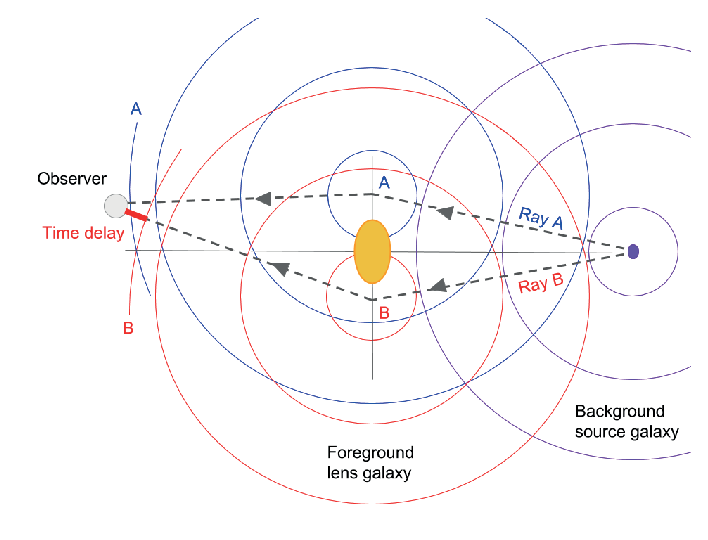
\includegraphics[scale=1.0]{pics/timedelayorigin.eps}
	\caption{Схематичная иллюстрация возникновения "геометрического" слагаемого в выражении для временной задержки. \label{fig:timedelayorigin} }
   \end{figure} 


Введём обозначение:
 
\begin{equation}\label{dDt}
D_{\Delta t} = \frac{D_{d} D_{s}}{D_{d s}} (1+z_1) 
\end{equation}

Нетрудно увидеть, что величина $D_{\Delta t}$ (которая иногда называется \textit{расстоянием временной задержки} (time-delay distance) обратно пропорциональна $H_0$, что видно из \eqref{ang_dia_dist}. Важно отметить множитель (1+$z_1$), который возникает из-за расширения Вселенной (временная задержка "происходит" на красном смещении $z_1$). Можно упростить уравнение \eqref{tau} следующим образом:

\begin{equation}\label{ef}
\tau(\boldsymbol{\theta}, \boldsymbol{\beta})=\frac{D_{\Delta t}}{c} \Phi(\boldsymbol{\theta},\boldsymbol{\beta}) \propto \frac{1}{H_0}\Phi(\boldsymbol{\theta},\boldsymbol{\beta}).
\end{equation}

Непосредственно $\tau(\boldsymbol{\theta}, \boldsymbol{\beta})$ не поддаётся измерению. Но зато можно измерить разницу этих величин для различных изображений.

\begin{equation}\label{dt}
\Delta \tau_{AB} = \tau(\boldsymbol{\theta}_A, \boldsymbol{\beta}) - \tau(\boldsymbol{\theta}_B, \boldsymbol{\beta}) \propto \frac{1}{H_0}\Delta \Phi_{AB}.
\end{equation}

%Knowledge of the lens mass distribution is of vital importance to the success of this cosmological inference: Equation 3 shows that the time delay distance is likely to be comparably sensitive to uncertainty in the predicted Fermat potential as it is to the measured time delay itself. More concentrated mass distributions with steeper density profiles produce longer time delays leading to shorter inferred time delay distances, and thus larger inferred values of H0 (Wucknitz, 2002; Kochanek, 2002; Suyu, 2012).

%Both α(θ) and ψ(θ) can be predicted given a model for the mass distribution of the lens.

Если смоделировать линзирующий потенциал $\Psi(\boldsymbol{\theta})$ и положение источника $\boldsymbol{\beta}$ (которое не наблюдается) и на основе этих данных рассчитать $\Delta \Phi_{AB}$, то можно использовать гравитационно линзирующие системы для вычисления постоянной Хаббла $H_0$ и других космологических параметров, например, безразмерные плотности материи $\Omega_m$ и тёмной энергии $\Omega_{\Lambda}$ (см. \eqref{ang_dia_dist}). Но зависимость $D_{\Delta t}$ от $H_0$ наиболее сильная, поэтому дальнейшее исследование посвящено именно этому параметру.

Отметим, что распределение массы в линзы подвержено ряду вырождений, самым существенным из которых является так называемое \nl{поискать название в русско-язычной лит-ре}"вырождение масса-плоскость" (mass-sheet degeneracy). Данное вырождение заключается в том, что существует такое преобразование модели распределения массы в линзе, при котором наблюдаемые величины - положения изображений источника, относительные усиления, видимые звездные величины (наблюдаемый поток) - остаются прежними, в то время, как временные задержки могут испытывать серьёзные изменения (\cite{falco1985}). Для снятия данного вырождение необходимо привлечение дополнительной информации о потенциале линзы. Например, моделированием динамики звёзд в галактике-линзе или изучением среды вдоль луча зрения
(\cite{suyu2010}).
 
Весь формализм выше описывает простую модель, в которой вся гравитирующая масса расположена в одной плоскости. Моделирование настоящих гравитационно линзирующих систем гораздо сложнее, но соотношение \eqref{dt} так или иначе возникает в ходе вычислений, поэтому зависимость от космологических параметров сохраняет свою форму. \nl{зачем этот абзац? при моделировании линзы все до сих пор пользуются приближением плоской линзы}

Для определения постоянной Хаббла по временной задержке между изображениями, блеск источника должен быть переменным. Разные его изображения, возникающие в результате гравитационного линзирования, будут изменять свой блеск также, как и источник, но с некоторой задержкой по времени. Измеряя временную задержку между изображениями одного и того же источника, можно получить значение постоянной Хаббла. Идея использования именно линзированных сверхновых для оценки $H_0$ была впервые предложена Сьюром Рефсдалом в 1964 году (\cite{refsdal1964}). \nl{повтор введения}

\chapter{Вычисление постоянной Хаббла по данным наблюдений SN Refsdal}

\section{Общие сведения о SN Refsdal}
\begin{figure}[H]
    \centering
	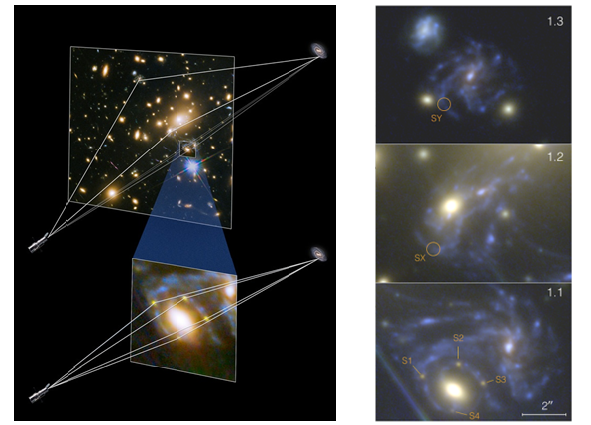
\includegraphics[width=0.9\linewidth]{pics/snrefsdal.png}
	\caption{\textit{Слева}: схематичное изображение хода лучей от SN Refsdal к  наблюдателю (источник: Space Telescope Science Institute). \textit{Справа}: изображения SN Refsdal (\cite{treu2016})}
	\label{fig:snrefsdalfig}
\end{figure}

Открытая в 2014 году в ходе обзора на телескопе \textit{Hubble Space Telescope} (\cite{kelly2014}) сверхновая SN Refsdal находится в рукаве спиральной галактики на красном смещении $z_s= 1.49$, которая линзируется скоплением галактик MACSJ1149.6+2223, находящимся на $z_d = 0.54$ таким образом, что существуют сразу три изображения родительской спиральной галактики (изображения 1.1, 1.2 и 1.3 на правой панели Рисунка \ref{fig:snrefsdalfig}). При этом в изображении 1.1 сверхновая дополнительно линзируется эллиптической галактикой скопления таким образом, что формируются четыре её изображения S1-S4 (правая нижняя панель Рисунка \ref{fig:snrefsdalfig}), расположенных в виде “креста Эйнштейна”. Изображение сверхновой SX (средняя панель справа) интересно тем, что его появление в 2015 году было предсказано с высокой точностью (\cite{kelly2014}, \cite{treu2016}). Согласно теоретическим оценкам, SY (правая верхняя панель) - это изображение сверхновой, которое “вспыхнуло” ~20 лет назад и уже угасло (\cite{kelly2014}, \cite{treu2016}).

%https://arxiv.org/pdf/1411.6009.pdf - appearance of refsdal
\section{Временные задержки и коэффициенты усиления}
Для определения постоянной Хаббла необходимы не только измерения временных задержек между различными изображениями, но и информация о гравитационном потенциале скопления, играющего роль линзы. На текущий момент представлен ряд моделей распределения вещества в скоплении галактик MACS J1149+2223, выступающего в роли линзы, разработанных разными коллективами авторов, и приведены теоретические предсказания временных задержек $\Delta t$ и коэффициентов усиления $\mu$ изображений S2, S3, S4, SX и SY относительно изображения S1 (\cite{treu2016}). Изображение SY далее не учитывается, так как оно не наблюдалось. В данной работе рассматриваются модели ‘Gri-g’, ‘Ogu-g’, ’Ogu-a’, ’Sha-g’, and ’Sha-a’, модели 'Die-a' и 'Zit-g' не учитываются\footnote{Названия моделей образованы первыми буквами фамилий руководителей команд, их разработавших: \textbf{Gri}llo, \textbf{Ogu}ri, \textbf{Sha}ron, \textbf{Die}go и \textbf{Zit}rin.}. Данные моделей подробно описаны в публикациях \cite{model_die}, \cite{model_gri}, \cite{model_ogu}, \cite{model_sha}, \cite{model_zit}. Предполагается, что $\Delta t$ и $\mu$ распределены нормально и не скоррелированы друг с другом, их средние значения и статистические погрешности приведены в Таблице \ref{tab:dtdm}.

\begin{table}[H]
 \caption{Рассматриваемые в этой работе временные задержки (в днях) и относительные усиления между изображениями SN Refsdal, предсказанные различными моделями распределения вещества \mbox{в скоплении галактик MACS J1149+2223 (\cite{treu2016}, Табл. 6).}}
 \label{tab:dtdm}
 \centering
 \scalebox{0.86}{
 \begin{tabular}{ | c | c | c | c | c | c | c | c | c |}
    \hline
    Модель & $\Delta t_{21}$ & $\Delta t_{31}$ & $\Delta t_{41}$ & $\Delta t_{X1}$ & $\mu_{21}$ & $\mu_{31}$ & $\mu_{41}$ & $\mu_{X1}$ \\ \hline
    Gri-g & $10.6^{+6.2}_{-3.0}$ & $4.8^{+3.2}_{-1.8}$ & $25.9^{+8.1}_{-4.3}$ & $361^{+19}_{-27}$ & $0.92^{+0.43}_{-0.52}$ & $0.99^{+0.52}_{-0.33}$ & $0.24^{+0.19}_{-0.20}$ & $0.36^{+0.11}_{-0.09}$ \\ \hline
    Ogu-g & $8.7 \pm 0.7$ & $5.1 \pm 0.5$ & $18.8 \pm 1.7$ & $311 \pm 24$ & $1.14 \pm 0.24$ & $1.22 \pm 0.24$ & $0.67 \pm 0.17$ & $0.27 \pm 0.05$ \\ \hline
    Ogu-a & $9.4 \pm 1.1$ & $5.6 \pm 0.5$ & $20.9 \pm 2.0$ & $336 \pm 21$ & $1.15 \pm 0.17$ & $1.19 \pm 0.17$ & $0.64 \pm 0.11$ & $0.27 \pm 0.03$ \\ \hline
    Sha-g & $6^{+6}_{-5}$ & $-1^{+7}_{-5}$ & $12^{+3}_{-3}$ & $277^{+11}_{-21}$ & $0.84^{+0.18}_{-0.06}$ & $1.68^{+0.55}_{-0.21}$ & $0.57^{+0.11}_{-0.04}$ & $0.25^{+0.05}_{-0.02}$ \\ \hline
    Sha-a & $8^{+7}_{-5}$ & $5^{+10}_{-7}$ & $17^{+6}_{-5}$ & $233^{+46}_{-13}$ & $0.84^{+0.20}_{-0.19}$ & $1.46^{+0.07}_{-0.49}$ & $0.44^{+0.05}_{-0.10}$ & $0.19^{+0.01}_{-0.04}$ \\ \hline
 \end{tabular}
 }
\end{table}

Как отмечалось выше, по кривым блеска сверхновой, наблюдаемым в различных изображениях, можно оценить относительную временную задержку. Кривые блеска SN Refsdal аппроксимировались кубическими сплайнами и различными полиномами (\cite{rodney2016}), однако, как отмечают авторы, использование существующей библиотеки шаблонов кривых блеска не позволяет воспроизвести все особенности кривой блеска SN Refsdal, поэтому их результаты требуют уточнения. В работе \cite{petrnat2020} построена физическая модель предсверхновой, удовлетворяющая фотометрическим наблюдениям в разных фильтрах. Это позволило уточнить значения временных запаздываний и коэффициентов усиления между изображениями SN Refsdal. Как и для моделей линз, представленных выше, предполагается, что $\Delta t$ и $\mu$ независимы и не коррелируют друг с другом, их значения приведены в Таблице \ref{tab:dtdmpetrnat}.

\begin{table}[H]
 \caption{Временные задержки (в днях) и относительные усиления между изображениями SN Refsdal, полученные из моделирования предсверхновой (\cite{petrnat2020}).}
 \label{tab:dtdmpetrnat}
 \centering
 \begin{tabular}{ | c | c | c | c | c | c | c | c |}
    \hline
    $\Delta t_{21}$ & $\Delta t_{31}$ & $\Delta t_{41}$ & $\Delta t_{X1}$ & $\mu_{21}$ & $\mu_{31}$ & $\mu_{41}$ & $\mu_{X1}$ \\ \hline
    $9.5^{+2.6}_{-2.7}$ & $4.2^{+2.3}_{-2.3}$ & $30.0^{+7.8}_{-8.2}$ & $340^{+43}_{-52}$ &  $1.14^{+0.02}_{-0.02}$ & $1.01^{+0.02}_{-0.02}$ & $0.35^{+0.016}_{-0.015}$ & $0.24^{+0.12}_{-0.07}$  \\ \hline
 \end{tabular}
\end{table}

%https://arxiv.org/pdf/2007.04106.pdf

% ноутбук по вычислению описанного выше
% https://colab.research.google.com/drive/1euY9KrqhSkNs0WtDz0o3tMGa5Wg6K3vZ#scrollTo=qG9K8eqFDprF
\section{Метод}
Для оценки постоянной Хаббла используется подход, предложенный в (\cite{vegaferrero}). Так как при построении моделей линзы (\cite{treu2016} (см. Табл. 6)) предполагалось, что постоянная Хаббла равна $H_0^{fid} = 70$ км с$^{-1}$ Мпк$^{-1}$, то значения временных задержек для каждой модели необходимо перемасштабировать таким образом, чтобы предсказанные значения наиболее точно совпали с наблюдаемыми. Логика этой операции проста: из выражения \eqref{ang_dia_dist} видно, что при прочих равных соотношение $H_0\Delta t$ остаётся постоянным. Перемасштабирование выполняется следующим образом:

\begin{equation}
p_{lens}(\Delta t, \mu | H_0, G) = p_{lens}(\frac{H_0^{fid}}{H_0} \Delta t, \mu | H_0^{fid}, G), 
\end{equation}

где $p_{lens}$  - вероятность того, что в отдельно взятой модели постоянная Хаббла примет значение $H_0$ при заданных $\Delta t$, $\mu$ между выбранными изображениями, а также распределении $G$ массы в гравитационной линзе. Далее применяется байесовский анализ: вероятность $P( H_0 |D)$ того, что постоянная Хаббла примет некоторое значение $H_0$ при заданных данных $D$, равна произведению априорной вероятности $P(H_0)$ на произведение распределений вероятности $p_{lens}(\Delta t, \mu| H0, G)$ для временных задержек и усилений в отдельно взятой модели линзы из (\cite{treu2016}) и $p_obs(\Delta t, \mu)$ в “наблюдаемых” данных (\cite{petrnat2020}): 

\begin{equation}
P( H_0 |D) \sim P(H_0) P( D | H_0 ) \sim P(H0) \int d \Delta t \ d \mu \ p_{lens}(\Delta t, \mu| H_0, G) \ p_{obs}(\Delta t, \mu).
\end{equation}
Вероятность в знаменателе формулы Байеса опускается, так как она постоянна для всех моделей.
\section{Результаты}



Распределения вероятности $P( H0 |D)$, рассчитанные по формуле (3) отдельно для пяти разных моделей, представлены на Рис. \ref{fig:probs}. 

\begin{figure}[H]
\begin{minipage}[h]{0.47\linewidth}
\center{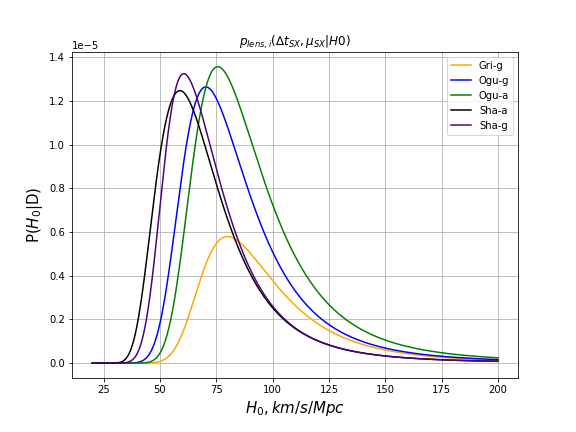
\includegraphics[width=1\linewidth]{hubbleconstant/picsforhubble/SX.png}} a) \\
\end{minipage}
\hfill
\begin{minipage}[h]{0.47\linewidth}
\center{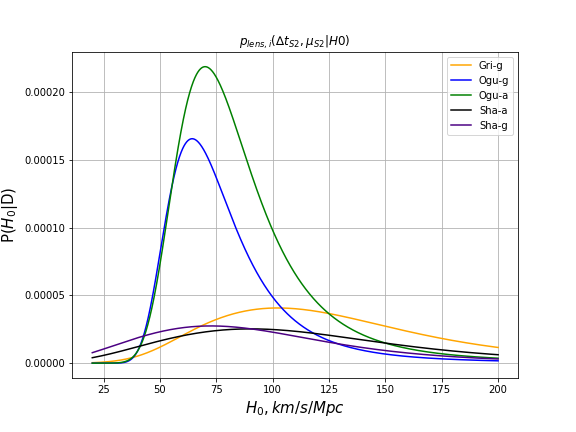
\includegraphics[width=1\linewidth]{hubbleconstant/picsforhubble/S2.png}} \\b)
\end{minipage}
\vfill
\begin{minipage}[h]{0.47\linewidth}
\center{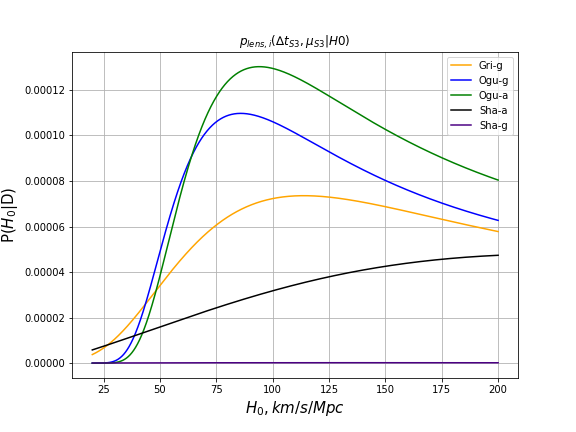
\includegraphics[width=1\linewidth]{hubbleconstant/picsforhubble/S3.png}} c) \\
\end{minipage}
\hfill
\begin{minipage}[h]{0.47\linewidth}
\center{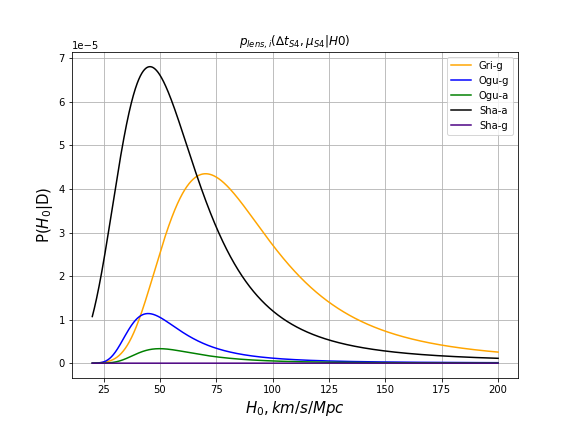
\includegraphics[width=1\linewidth]{hubbleconstant/picsforhubble/S4.png}} d) \\
\end{minipage}
\caption{Вероятность $P( H0 |D)$, вычисленная по формуле (3) для пар изображений SX-S1, S2-S1, S3-S1, S4-S1 (слева направо, сверху вниз). Амплитуда (в относительных единицах) пика указывает на то, насколько хорошо согласуются предсказания усилений, полученных из теоретической модели линзы, с наблюдениями.}
\label{fig:probs}
\end{figure}



Отдельные значения вероятности моделей были сложены с одинаковыми весами. Таким образом были получены распределения $P_+( H0 |D)$ величины постоянной Хаббла, изображенные на Рис. \ref{fig:sumprobs}.

\begin{figure}[H]
\begin{minipage}[h]{0.47\linewidth}
\center{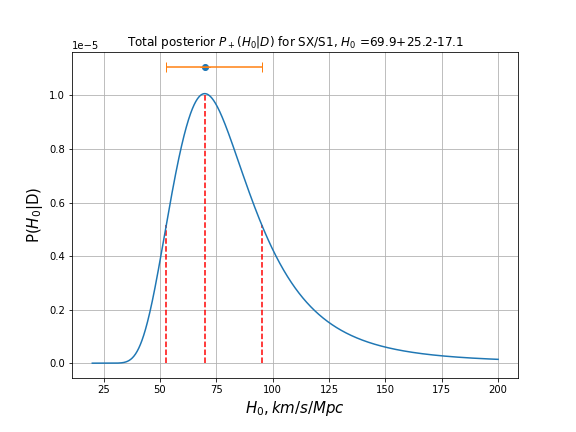
\includegraphics[width=1\linewidth]{hubbleconstant/picsforhubble/H_0 - SX.png}} a) \\
\end{minipage}
\hfill
\begin{minipage}[h]{0.47\linewidth}
\center{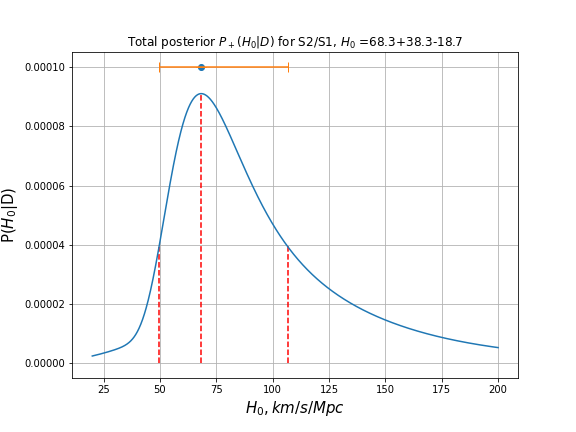
\includegraphics[width=1\linewidth]{hubbleconstant/picsforhubble/H_0 - S2.png}} \\b)
\end{minipage}
\vfill
\begin{minipage}[h]{0.47\linewidth}
\center{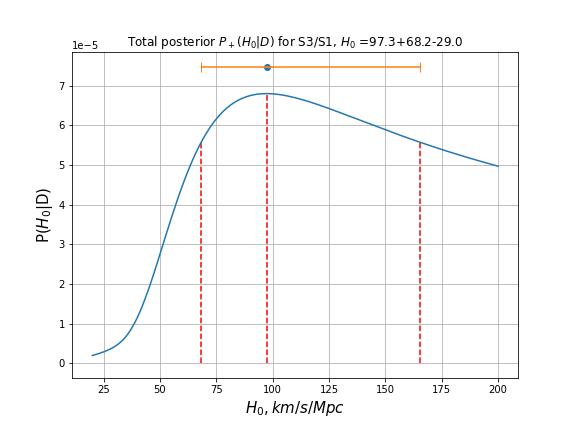
\includegraphics[width=1\linewidth]{hubbleconstant/picsforhubble/H_0 - S3.png}} c) \\
\end{minipage}
\hfill
\begin{minipage}[h]{0.47\linewidth}
\center{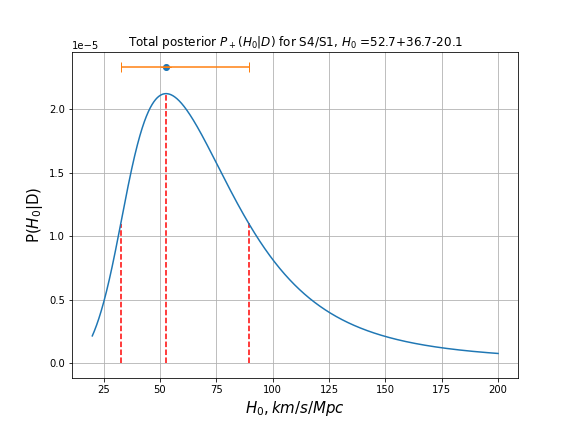
\includegraphics[width=1\linewidth]{hubbleconstant/picsforhubble/H_0 - S4.png}} d) \\
\end{minipage}
\caption{Сумма вероятностей $P_{+}( H_0 |D)$, вычисленных по формуле (3), по всем моделям. В данной работе ошибки рассчитаны относительно пика распределения.}
\label{fig:sumprobs}
\end{figure}




Поскольку область с изображениями S1-S4 находится далеко от области с изображением SX, можно считать, что гравитационные потенциалы в этих областях никак не связаны. Для уменьшения статистических ошибок можно использовать два изображения, которые можно считать нескоррелированными. Поэтому дополнительно значение $H_0$ было рассчитано по комбинации значений, полученных по изображениям S2 и SX. Такой выбор обусловлен тем, что наиболее жёсткие ограничения (то есть самые маленькие ошибки) на временную задержку среди изображений S2, S3, S4 - в изображении S2, как следствие, постоянная Хаббла, вычисленная по ней, будет иметь самые маленькие ошибки. Комбинированная апостериорная вероятность для пары изображений SX-S2 в отдельно взятой модели $i$ вычислялась как

\begin{equation}
p_{lens, i}(\Delta t_{S2},\mu_{S2}|H_0) × p_{lens,i}(\Delta t_{SX}, \mu_{SX}|H_0),
\end{equation}

\noindent после чего полученные значения суммировались с равными для каждой модели весами. Полученные результаты представлены на Рис. \ref{fig:probs2}. Согласно таким оценкам, значение постоянной Хаббла равно $H_0=71.2_ {-11.6}^{+16.4}$. При увеличении числа рассматриваемых гравитационно-линзированных систем можно существенно улучшить ошибки величины $H_0$.

\begin{figure}[h]
\begin{minipage}[h]{0.49\linewidth}
\center{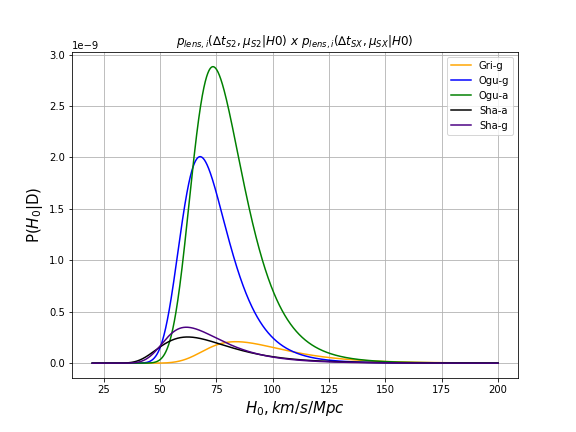
\includegraphics[width=0.99\linewidth]{hubbleconstant/picsforhubble/SX+S2.png}}
\end{minipage}
\hfill
\begin{minipage}[h]{0.49\linewidth}
\center{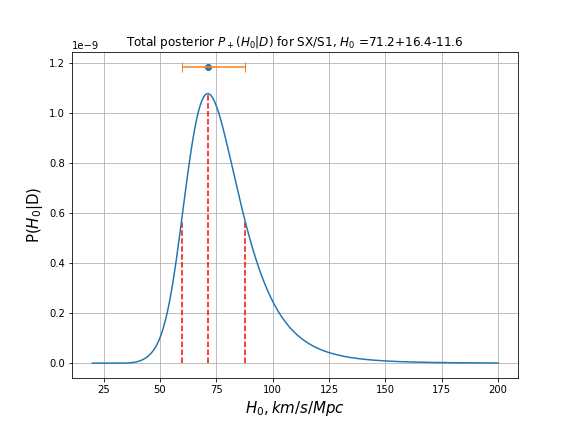
\includegraphics[width=0.99\linewidth]{hubbleconstant/picsforhubble/H_0 - SX+S2.png}}
\end{minipage}
\caption{Слева: $P( H0 |D)$ для изображений SX и S2 для отдельно взятых моделей, рассчитанная по формуле (4). Справа: сумма вероятностей $P_{+}( H0 |D)$ по всем моделям.}
\label{fig:probs2}
\end{figure}



\section{Обсуждение}

На основе сравнения прогнозов временных задержек и коэффициентов усиления, рассчитанных в различных моделях гравитационного потенциала линзы-галактики и масштабированных таким образом, чтобы они совпадали с наблюдаемыми величинами, вычислено значение постоянной Хаббла, наиболее точно удовлетворяющее и модельным, и наблюдательным данным: $H_0=71.2_ {-11.6}^{+16.4}$ . Для уменьшения статистических ошибок это значение было рассчитано по нескольким изображениям сверхновой SN Refsdal. Существенно улучшить оценку $H_0$ поможет увеличение числа рассматриваемых систем. Полученные результаты также могут послужить независимым тестом различных  моделей распределения масс в линзе-галактике. Также следует отметить, что при вычислениях не учитывалось влияние микролинзирования. Этот эффект рассмотрен в следующем разделе.


\chapter{Микролинзирование}\label{ch:micro}

\section{Общие сведения о микролинзировании}
При детальном анализе временной задержки между изображениями гравитационно линзированных сверхновых нельзя пренебречь \textit{микролинзированием} - линзированием на отдельных звёздах или других компактных объектах в галактике-линзе. Его масштабы, то есть характерные углы отклонения света, в миллион раз меньше масштабов сильного линзирования. На текущий момент разрешить множественные изображения, возникающие в результате микролинзирования не представляется возможным. Однако вполне возможно “засечь” этот эффект благодаря кратковременному увеличению или ослаблению яркости источника. Микролинзирование не вносит существенный вклад в наблюдаемую кривую блеска, если размер источника сильно превышает радиус Эйнштейна $\theta_E$ для звезды-микролинзы. Напомним, что эта величина задаётся соотношением:

\begin{equation}\tag{\ref{eq:r_ein}}
\theta_{E}=\sqrt{\frac{4 G M}{c^{2}} \frac{D_{d s}}{D_{d} D_{s}}}.
\end{equation}

Известно, что для источников с угловым размером $\theta > 5\theta_E$ значение обусловленной микролинзированием добавки к звёздной величине обратно пропорционально $\theta$ (\cite{refsdalstabell1991}). Для конфигурации SN Refsdal оценим $\theta_E$ для звезды с массой $1 M_{\odot}$. Расстояния до галактики-линзы (члена скопления MACSJ1149.6+2223, $z_d=0.54$), до источника ($z_Ss=1.49$), а также между линзой и источником равны, согласно формуле \eqref{eq:ang_dia_dist}, 
$$ D_d=D_A(0,z_d)=1311.54 \ \textrm{МПк}, $$
$$ D_s=D_A(0,z_s)=1744.81 \ \textrm{МПк}, $$
$$ D_{ds}=D_A(z_d,z_s)=932.47 \ \textrm{МПк}, $$
соответственно. В результате, радиус Эйнштейна для звезды с массой $1 M_{\odot}$ составляет, согласно формуле \eqref{eq:r_ein}, $$\theta_E \approx 1.8 \cdot 10^{-6} \ ''. $$ 

Для сверхновых II типа максимальный размер фотосферы составляет $R_{SN} \sim 10^{15}$ см (\cite{razmer}). По результатам гидродинамического моделирования расширения оболочки SN Refsdal её максимальный размер составляет $R_{SN} = 1.75\cdot10^{15}$ см (\cite{petrnat2020}), или, в угловых единицах, $$\theta_{SN} = \frac{R_{SN}}{D_S} \approx 6.7 \cdot 10^{-8} \ '' =  0.037 \cdot \theta_E $$  Таким образом, угловой размер SN Refsdal не превышает характерный радиус Эйнштейна, а значит, микролинзирование может вносить существенные искажения в её кривые блеска. %Эта оценка пригодится нам немного позже для оценки масштаба карт.

В данной работе для изучения микролинзирования используется вычислительная программа {\tt{microlens}} (\cite{wambsganss1990-thesis}, \cite{wambsganss1999}), которая моделирует методом обратной трассировки лучей (\textit{inverse ray shooting}, \cite{kayserrefsdal1986}) распределение каустик в плоскости источника, основываясь на распределении звёзд в плоскости линзы. Выходными данными этой программы являются карты микрокаустик - двумерные массивы, каждый пиксель которых содержит значения обусловленного микролинзированием усиления в плоскости источника. Основными входными параметрами для каждой карты являются безразмерные поверхностные плотности звёзд $\kappa_*$ и непрерывно распределенной тёмной материи $\kappa_c$ в линзирующей галактике\footnote{Либо параметр $s=\kappa_c/(\kappa_*+\kappa_c)$.}, внешний сдвиг $\gamma$, учитывающий вклад гравитационного потенциала скопления галактик, а также функция масс звёзд. 

%Dobler, Keeton 2006

%Several authors have shown that microlensing magnification distributions are insensitive to the mean mass ¯m (Wyithe & Turner 2001; Schechter et al. 2004; Mortonson et al. 2004). For microlensing of SN light curves, the mean mass does set an overall time scale: as ¯m increases, the time it takes for the source to reach a given fraction of R¯ scales as ¯m1/2

%The properties of the microlensing fluctuations should be dependent on the stellar population parameters (namely f∗ and q). They also depend on the particular configuration of stars, because as shown in Figure 2 different realizations of stellar populations that are statistically equivalent yield very different magnification maps in the source plane. Note that these magnification maps are 2.5R¯ on a side, so a SN will expand to cover roughly half of a map during its observable lifetime.

Здесь и далее предполагается, что все звезды в галактике имеют одинаковую массу, которая равна массе Солнца $M_{\odot}$. Вопрос о допустимости этого предположения остаётся открытым, по данным некоторых исследований эффект микролинзирования слабо зависит от начальной функции масс ((\cite{refsdalstabell1991}, \cite{doblerkeeton2006}, \cite{hubersuyu2019}, \cite{goldstein2018}). Также предполагается, что значения карт усилений не изменяются на характерных временах расширения сверхновой, то есть эффект от микролинзирования связан только с пространственным расширением сверхновой, но не с динамикой звёзд в галактике-линзе.

%На Рисунке \ref{fig:micromaps} приведены примеры результатов выполнения программы {\tt{microlens}} - карты усилений для двух различных значений количества звёзд, вызывающих микролинзирование. Светлые области означают, что источник усиливается, находясь в них, тёмные - что ослабляется. Видно, что а) сеть каустик намного богаче при большем количестве звёзд-линз, б) по всей карте усиление меняется и почти нигде не остаётся таким, каким его предсказывает модель линзы, то есть в отсутствие микролинзирования.

%\begin{figure}[H]
%    \centering
%	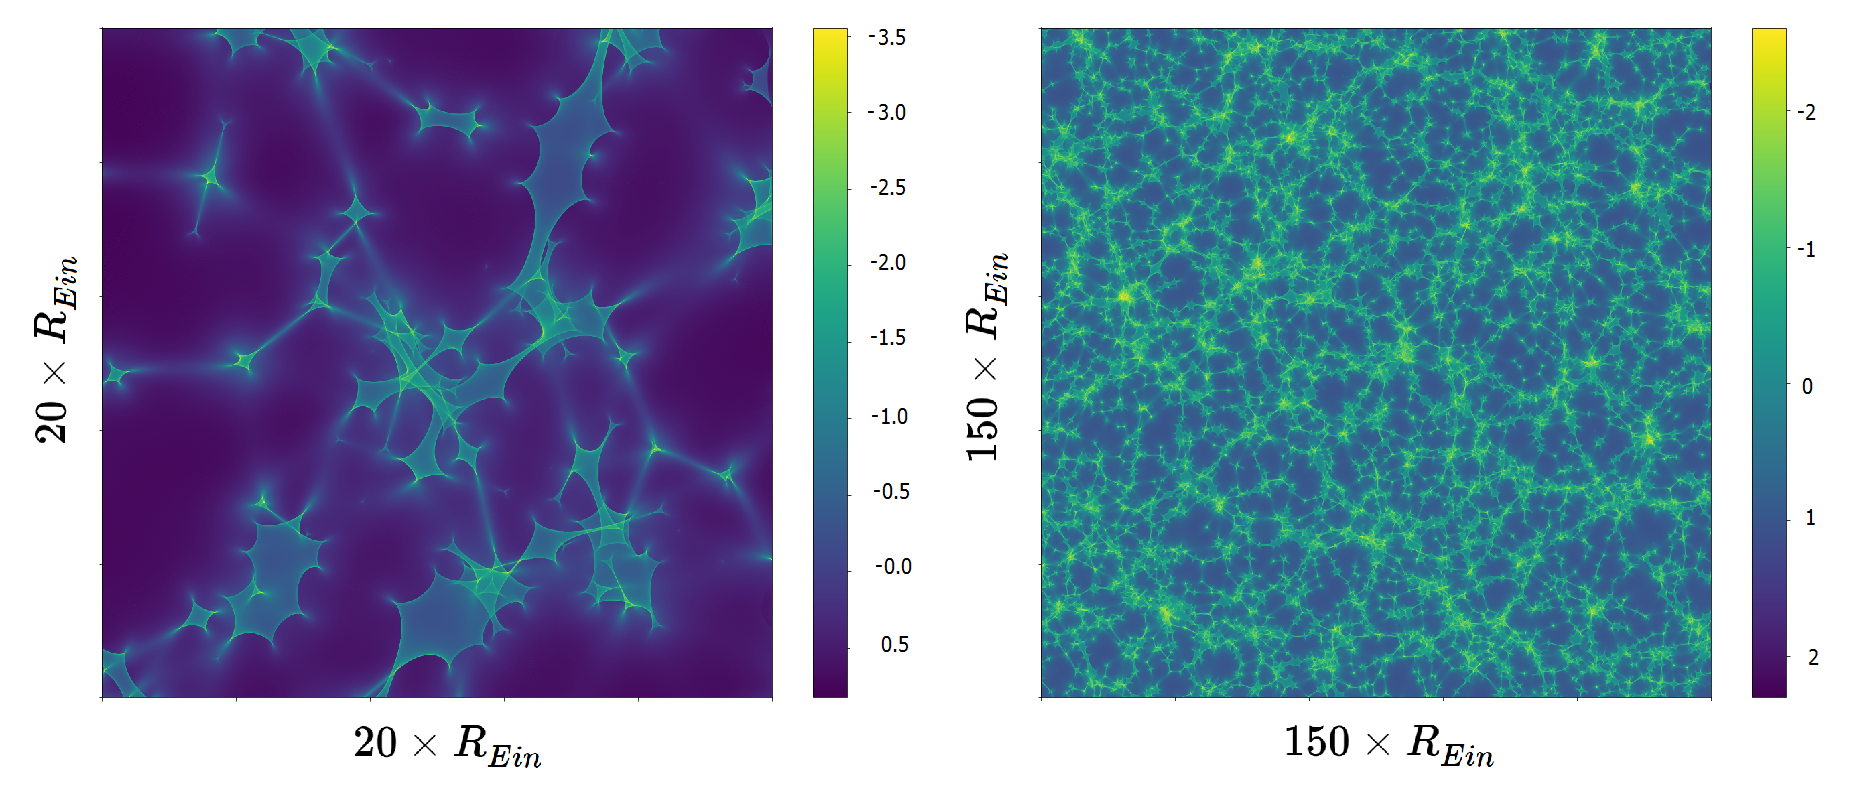
\includegraphics[scale=0.22]{pics/maps_example.png}
%	\caption{Карты микрокаустик. Количество звёзд-линз слева - 313, справа - 14526. Цветовая шкала (в единицах звёздных величин) показывает, как дополнительно увеличивается или ослабляется яркость источника вследствие только микролинзирования. \label{fig:micromaps}} 
%\end{figure}


\section*{Оценки $\kappa_*, \kappa_c$ и $\gamma$ для изображений SN Refsdal}
Для того чтобы охарактеризовать степень влияния микролинзирования на кривые блеска SN Refsdal, необходимо оценить параметры галактики-линзы, ответственной за появление изображений S1-S4, а именно локальные значения параметров $\kappa_*, \kappa_c$ и $\gamma$ в областях изображений S1-S4  (см. Рис. \ref{fig:snrefsdalfig}). Параметры $\kappa$ и $\gamma$ известны из модели скопления MACSJ1149.6+2223 (\cite{treu2016}, а также ссылки в ней; \cite{hubblemaps}). Здесь и далее мы будем придерживаться модели линзы\footnote{Mодели размещены на сайте \cite{https://archive.stsci.edu/pub/hlsp/frontier/macs1149/models/}.}, подробно описанной в работе \cite{kawamataoguri}. Используемые значения $\kappa$ и $\gamma$ для изображений S1-S4 приведены в Табл. \ref{tab:kappagamma}.
\begin{table}[h!]
  \caption{$\kappa$, $\gamma$ в областях изображений SN Refsdal} 
  \label{tab:kappagamma}
  \centering
    \begin{tabular}{ | c | c | c | c | c |}
    \hline
    Изображение & S1 & S2 & S3 & S4 \\ \hline
    $\kappa$ & 0.728 & 0.725 & 0.670 & 0.744 \\ \hline
    $\gamma$ & 0.108 & 0.347 & 0.221 & 0.484 \\
    \hline
    \end{tabular}
\end{table}
Так как в качестве галактики-линзы, ответственной за появление изображений S1-S4, выступает эллиптическая галактика, то оценка $\kappa_*$, то есть вклада в микролинзирование именно звёзд, может быть получена на основе эмпирических корреляций между основными свойствами эллиптических галактик: эффективным радиусом $r_e$, эффективной поверхностной плотностью звёзд $\Sigma_e$ и дисперсией скоростей звёзд $\sigma$. Эта зависимость известна как \textit{фундаментальная плоскость} (\cite{djorgovski&davis1987}, \cite{hydebernardi2009}). Также известно, что для эллиптических галактик поверхностная яркость (а значит, и поверхностная плотность звёзд) связана с расстоянием от её центра по закону де Вокулёра (\cite{vaucouleurs}). Для оценки $\kappa_*$ и $\kappa_c$ в областях изображений сверхновой Рефсдала мы следуем подходу, детально описанному в работе \cite{schechter2014}, суть которого состоит в том, что фундаментальная плоскость записывается в терминах эффективной поверхностной плотности $\Sigma_{e}$, эффективного радиуса $r_e$ и дисперсии скоростей звёзд в галактике-линзе, которая определяется следующим образом:

\begin{equation}\label{sigrad}
\log \Sigma_{e}=A \log \left(\frac{\sigma_{p r o x}}{265  \mathrm{km} / \mathrm{s}}\right)+C, \ \ \ \ \ \ \ \log r_{e}=D \log \left(\frac{\sigma_{\text {prox}}}{265 \mathrm{km} / \mathrm{s}}\right)+E,
\end{equation}

\begin{equation}\label{sigmaprox}
\textrm{где} \ \sigma_{prox}=c \sqrt{\frac{\theta_{\text {Ein}}}{4 \pi} \frac{D_{ds}}{D_{s}}},
\end{equation}
$\theta_{\text {Ein}}$ -- радиус Эйнштейна для линзирующей галактики. Для галактик-линз на красном смещении $z \sim 0.2$ путём интерполяции данных из обзора SLACS получены значения коэффициентов (\cite{schechter2014}): $$ A = -1.702, \ C = 9.156, \ D = 2.401, \ E = 0.832. $$ Несмотря на то, что галактика, ответственная за появление изображений S1-S4 SN Refsdal, находится на $z \sim 0.5$, существенной эволюции этих параметров не ожидается (\cite{2013ApJ...779L..21B}). Поскольку значение $\theta_{\text {Ein}}$ неизвестно, воспользуемся следующим значением дисперсии скоростей звёзд для галактики-линзы: $\sigma_{prox} \simeq 232$ км/с (\cite{kawamataoguri}). %Ожидается, что оно лежит достаточно близко к $\sigma_{prox}$. 
Подставляя указанное  значение $\sigma_{prox}$ в формулы \eqref{sigrad}, получаем: $$\Sigma_e = 1.8 \cdot 10^9 \ M_{\odot}/pc^2, \ \ \ \ \ r_e=4.93 \ kpc$$
В работе \cite{kawamataoguri} приведены положения (в системе небесных координат) изображений S1-S4 (Таблица А4) и центра линзирующей галактики (раздел 3.4.4), они указаны в таблице \ref{tab:coord}.

\begin{table}[h!]
  \caption{Координаты изображений SN Refsdal и галактики-линзы (\cite{kawamataoguri})}
  \label{tab:coord}
  \centering
    \begin{tabular}{ | c | c | c | c | c |}
    \hline
     & Прямое восхождение & Склонение \\ \hline
    S1 & 177.398225 & 22.395628 \\ \hline
    S2 & 177.397713 & 22.395781 \\\hline
    S3 & 177.397371 & 22.395531 \\ \hline
    S4 & 177.3978   & 22.395181 \\\hline
    Галактика-линза & 177.397842 & 22.395591 \\\hline
    \end{tabular}
\end{table}

Поверхностная плотность звёзд $\Sigma_*$ в областях, соответствующим изображениям S1-S4, рассчитывается на основе формулы де Вокулёра (\cite{vaucouleurs}), представленной в виде (\cite{schechter2014}, формула (11)):

\begin{equation}\label{vaucouleurs}
\Sigma_*\left(u_{i}, v_{i}\right)=\mathcal{F} \frac{\Sigma_{e}}{3.607} \exp \left[-\left(\frac{w_{i}}{r_{e}}\right)^{\frac{1}{4}}+1\right], 
\end{equation}
где $u_{i}, v_{i}$ - координаты $i$-ого изображения по отношению к центру линзирующей галактики, $\Sigma_e$ - средняя (эффективная) поверхностная плотность звёзд, заключённых внутри эффективного радиуса $r_e$, безразмерный множитель $\mathcal{F}=1.23$ подобран методом максимального правдоподобия по наблюдаемым световым потокам от квазаров. При этом, согласно формуле \eqref{eq:convergence} для плоскости, в которой находятся изображения SN Refsdal  $\Sigma_{crit} = 2371.9 \ M_{\odot}/pc^2 $. Располагая этим значением, можно также найти $\kappa_*$ и $\kappa_c$ для областей с изображениями S1-S4 ($\kappa_*=\Sigma_* /\Sigma_{crit}, \ \kappa_c = \kappa-\kappa_* $). Полученные результаты представлены в таблице \ref{tab:paramsfors1234}.

\begin{table}[H]
 \caption{Оценки параметров для изображений SN Refsdal}
 \label{tab:paramsfors1234}
 \centering
 \begin{tabular}{ | c | c | c | c | c |}
    \hline
    Изображение & S1 & S2 & S3 & S4 \\ \hline
    $\Sigma_*, M_{\odot}/pc^2$ & 491.2 & 541.3 & 509.8 & 580.1\\ \hline
    $\kappa_*$ & 0.207 &  0.228 & 0.215 & 0.245 \\ \hline
    $\kappa_c$ & 0.521 & 0.496 & 0.455 & 0.499 \\ \hline
    $\kappa_*/\kappa$ & 0.285 & 0.315 & 0.321 & 0.329 \\ \hline
 \end{tabular}
\end{table}

%Реализации карт с соответствующими параметрами приведены на Рисунке \ref{fig:s1s4}.

%\begin{figure}[H]
%    \centering
%	\includegraphics[scale=0.6]{pics/s1s4.png}
%	\caption{Реализации карт для областей изображений S1-S4 SN Refsdal, выполненные при помощи программы {\tt{microlens}}. Размер каждой карты -- $10 \times 10 \ R_{Ein} $, разрешение -- $1000 \times 1000 $ пикселей. Цветовая шкала в единицах звёздных величин показывает усиление (отрицательные значения) или ослабление (положительные значения) яркости источника вследствие только микролинзирования. \label{fig:s1s4}} 
%\end{figure}

\section{Карты усилений}
%Первоочерёдной задачей при анализе влияния микролинзирования на кривые блеска SN Refsdal является оценка параметров галактики-линзы, ответственной за появление изображений S1-S4 (см. Рис. \ref{fig:snrefsdalfig}). На основе эмпирических соотношений для основных свойств эллиптических галактик - эффективного радиуса $r_e$, эффективной поверхностной плотности $\Sigma_e$ и дисперсии скоростей звёзд $\sigma_{prox}$ (\cite{schechter2014}, - а также закона де Вокулёра (\cite{vaucouleurs}), который связывает поверхностную яркость в эллиптической галактике с расстоянием до её центра, была проведена оценка $\kappa*$, $\kappa_c$ и $\gamma$ в областях, в которых находятся изображения S1-S4 SN Refsdal, координаты которых относительно центра эллиптической галактики известны из работы \cite{kawamataoguri}, и на основе этого построены карты усилений для этих областей. Детальный вывод вышеупомянутых параметров представлен в Приложении. \textbf{Или лучше пусть здесь будет?} 

%Локальные значения параметров $\kappa_*, \kappa_c$ и $\gamma$ в областях изображений S1-S4 представлены в Таблице \ref{tab:allparamsfors1234}.

%\begin{table}[H]
%  \caption{Оценки параметров для изображений SN Refsdal}
%   \label{tab:allparamsfors1234}
%  \centering
%    \begin{tabular}{ | c | c | c | c | c |}
%    \hline
%    Изображение & S1 & S2 & S3 & S4 \\ \hline
%    $\kappa$ & 0.728 & 0.725 & 0.670 & 0.744 \\ \hline
%    $\gamma$ & 0.108 & 0.347 & 0.221 & 0.484 \\ \hline
%    $\Sigma_*, M_{\odot}/pc^2$ & 491.2 & 541.3 & 509.8 & 580.1\\ \hline
%    $\kappa_*$ & 0.207 &  0.228 & 0.215 & 0.245 \\ \hline
%    $\kappa_c$ & 0.521 & 0.496 & 0.455 & 0.499 \\ \hline
%    $\kappa_*/\kappa$ & 0.285 & 0.315 & 0.321 & 0.329 \\ \hline
%    \end{tabular}
%\end{table}

В данной работе анализируются кривые блеска SN Refsdal, наблюдаемые в изображениях S1 и S2, так как временная задержка между ними рассчитана с наименьшими погрешностями. Для набора параметров, характеризующих области этих изображений, в программе \texttt{microlens} построены карты микролинзирования. Они изображены на Рисунке \ref{fig:mymaps}, размер каждой карты - $5\times5$ радиусов Эйнштейна в плоскости источника, разрешение - $10000\times10000$ пикселей. Выбор такого масштаба (1 радиус Эйнштейна = 2000 пикселей) обусловлен необходимостью задания профиля яркости сверхновой на большом количестве точек вдоль радиуса. В рамках проверки корректности полученных карт проведено их статистическое исследование. Гистограммы по их значениям сравниваются с гистограммами карт с аналогичными параметрами из обзора \texttt{GERLUMPH} (\cite{gerlumph}). Эти карты получены независимой командой исследователей и лежат в открытом доступе. Кроме того, на гистограммы также нанесена зависимость $\mu^{-3}$, которой подчиняется усиление точечных источников для больших $\mu$ (\cite{wambsganss1992-probabilities}, \cite{blandfordnarayan1986}). Максимальный радиус SN Refsdal на этих картах – 72 пикселя. Предполагается, что при таком масштабе станет возможным различить флуктуации микролинзирования от источников с плоским и гауссовым профилями яркости. На Рисунке \ref{fig:mymaps} изображены полученные карты и построенные по ним гистограммы. Светлые области означают, что точечный источник усиливается, находясь в них, тёмные - что ослабляется. Видно, что а) сеть каустик отличается в зависимости от входных параметров, б) практически по всей карте усиление меняется и почти нигде не остаётся таким, каким его предсказывает модель линзы, то есть в отсутствие микролинзирования.

\begin{figure}[H]
    \centering
	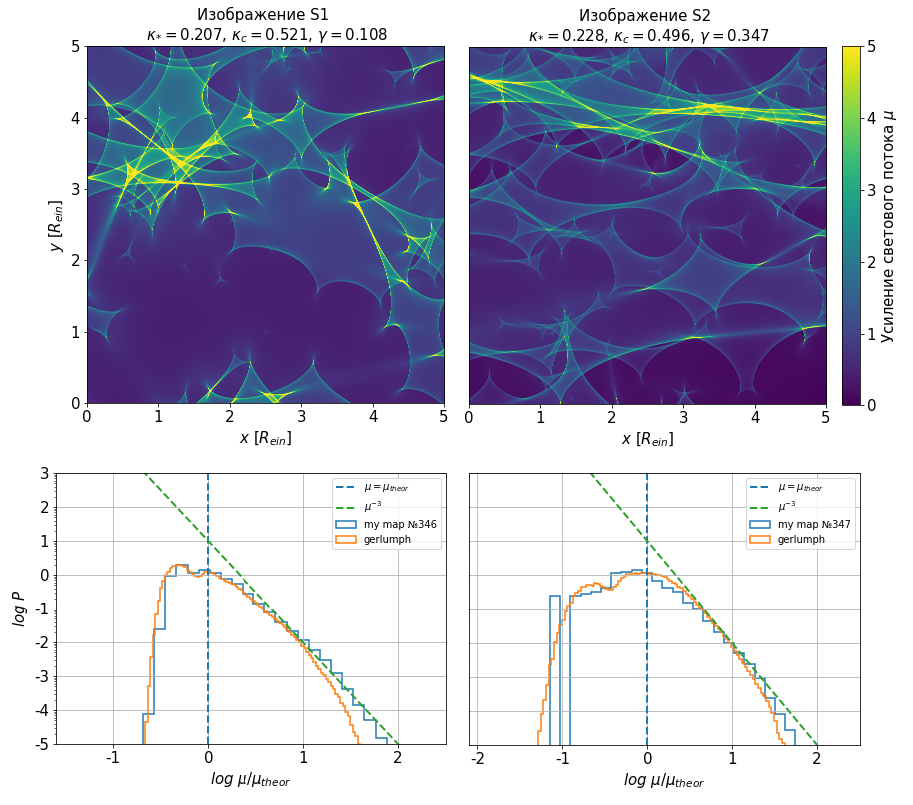
\includegraphics[width=\textwidth]{microlensing/images/mapsandhistS12.png}
	\caption{Сверху: Карты усилений, вызванных микролинзированием, в областях изображений S1 (слева) и S2 (справа) SN Refsdal. Значения усилений ограничены сверху для контраста, в действительности в некоторых областях значение абсолютных усилений может достигать нескольких десятков. Снизу: гистограммы по этим картам и по картам из обзора GERLUMPH с теми же параметрами. На гистограммы нанесена теоретическая вероятность $P(\mu)\propto \mu^{-3}$ в пределе больших усилений $\mu$ (зелёная пунктирная линия) и теоретическое значение усиления в отсутствие микролинзирования (синяя пунктирная линия).}
	\label{fig:mymaps}
\end{figure}


Теоретическое макро-усиление карты (другими словами, среднее усиление по карте) зависит от параметров $\kappa$ и $\gamma$ и определяется ранее указанной формулой:

\begin{equation}\tag{\ref{eq:magnification}}
\mu_{th} = \frac{1}{(1-\kappa)^2-\gamma^2}.
\end{equation}

Среднее численное усиление карты задаётся формулой

\begin{equation}\label{avmag}
\mu_{num} = \frac{1}{N_{pix}^2}\sum_{i,j=1}^{n_{pix}}\mu_{ij} \ ,
\end{equation}

\noindent где $N_{pix}$ - сторона карты в пикселях, $\mu_{ij}$ - усиление пикселя с координатами $(i,j)$. Значения $\mu_{th}$ и $\mu_{num}$, как правило, в точности не равны друг другу, так как параметры, по которым построена карта, описывают гораздо большую область, чем та, для которой эта карта построена. Таким образом, средняя поверхностная плотность массы внутри региона, для которого построена карта, может быть больше или меньше, чем та что использовалась в качестве входного параметра. Кроме того, численное и теоретическое усиление могут не совпадать в силу того, что характерный размер некоторых каустик больше, чем размер карты, то есть поле карты слишком мало, чтобы продемонстрировать характерное поведение микролинзирования для заданных параметров (\cite{wambsganss1990-thesis}). 

% док с анализом карт
% https://docs.google.com/document/d/13IuvRnhXnfZHm1f0Ig94AjY7qQ2oOU3txVK2iy2Xmq8/edit#heading=h.sdu2d5mkt4xj
\section{Учёт протяженности источника}
В данной работе расширяющаяся сверхновая аппроксимируется расширяющимся кружком с заданным симметричным профилем поверхностной яркости. Как можно получить значение обусловленной микролинзированием вариации блеска в фиксированный момент времени, то есть для заданного радиуса кружка? Известна следующая формула: наблюдаемый поток $F_{\lambda}(\lambda,t)$ от источника на длине волны $\lambda$ и в момент времени $t$ получается в результате свёртки зависящей от времени яркости кружка-сверхновой $I_{\lambda}(P,\phi,\lambda, t)$ с "накрываемым" \ им участком усилений карты микролинзирования $\mu(P,\phi)$ в плоскости, перпендикулярной к лучу зрения (\cite{goldstein2018}, \cite{hubersuyu2019}). Так как модель сферически-симметричная, получается, что

\begin{equation}\label{eq:eft}
F_{\lambda}(\lambda,t) = D_L^{-2} \int_0^{2\pi} \int_0^{P_m} I_{\lambda}(P,\phi,\lambda, t) \mu(P,\phi)P dP d\phi,
\end{equation}

\noindent где $\phi$ и $P$ являются азимутальным и прицельным параметрами (полярными координатами точек), $D_L$ - болометрическое расстояние\footnote{Оно связано с расстоянием углового диаметра $D_A$ следующим образом: $D_L = (1+z)^2 D_A$ (\cite{distance_measures}).} (\textit{luminosity distance}) до сверхновой, $P_m$ - максимальный прицельный параметр. Формула \eqref{eq:eft} проиллюстрирована на Рисунке \ref{fig:goldsteinn}. 

\begin{figure}
    \centering
	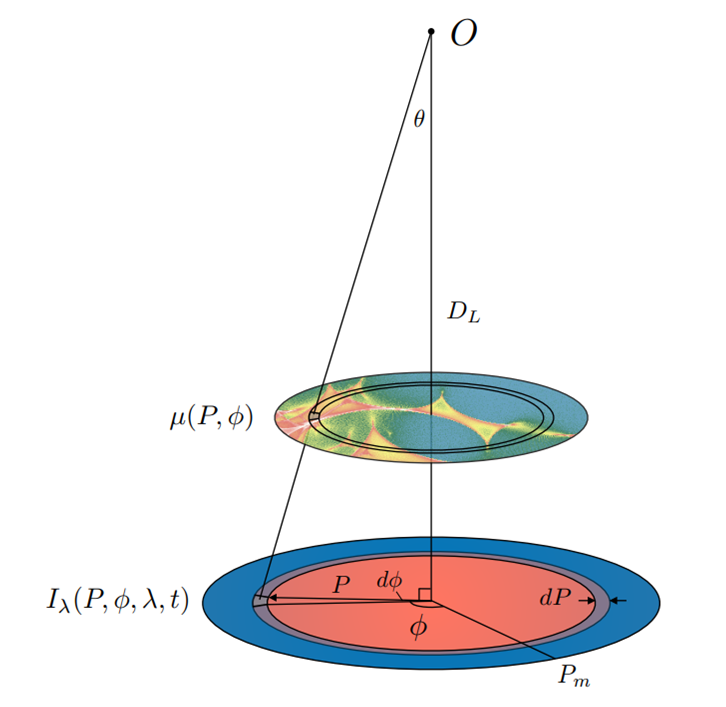
\includegraphics[scale=0.77]{microlensing/images/goldstein.png}
	\caption{Иллюстрация свертки источника с картой (\cite{goldstein2018})} 
	 \label{fig:goldsteinn}
\end{figure}

Сверхновая моделировалась кругом, который расширяется со скоростью $v=500$ км/с в течение 160 дней (в её системе отсчёта). Выбор такого значения скорости обусловлен результатами, полученными при моделировании радиуса фотосферы SN Refsdal (\cite{petrnat2020}). График зависимости радиуса фотосферы от времени приведен на Рисунке \ref{fig:snexpand}.

\begin{figure}[H]
    \centering
	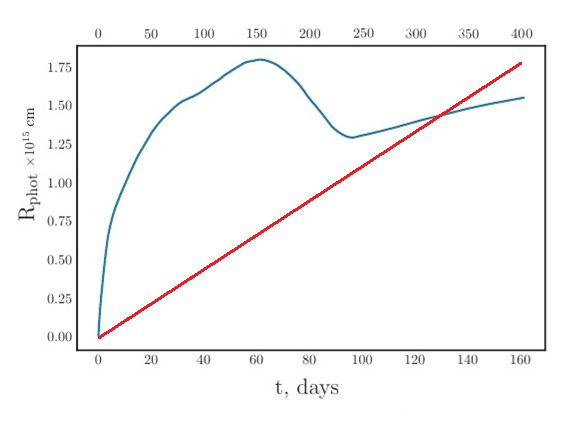
\includegraphics[width=0.8\textwidth]{microlensing/images/snexpand.png}
	\caption{Синий цвет: эволюция радиуса фотосферы $R_{phot}$ в модельном расчёте вспышки сверхновой (\cite{petrnat2020}). Красный цвет: аппроксимация, принятая в данной работе. По горизонтальной оси отложены две временные шкалы: в системе отсчёта сверхновой (снизу) и в системе отсчёта наблюдателя (сверху). Эти шкалы связаны друг с другом множителем $(1+z_{s})\approx 2.5$.}
	\label{fig:snexpand}
\end{figure}

\newpage

Значение абсолютного усиления получается делением потока от кружка-сверхновой, свёрнутого с картой усилений, на значение потока при отсутствии микролинзирования (формула \ref{eq:eft} с $\mu(P,\phi)=1$). Вклад в кривую блеска, обусловленный только микролинзированием, выраженный в звёздных величинах, задаётся выражением:

\begin{equation}\label{eq:deltam}
\Delta m (t)= - 2.5\log \Big[ \frac{L(t)}{S(t)} \Big],
\end{equation}

\begin{equation}\label{eq:iott}
\textrm{где} \ L(t) = \int_0^{2\pi} \int_0^{P_m} I_{\lambda}(P,\phi,\lambda, t) \mu(P,\phi)P dP d\phi
\end{equation}

\begin{equation}\label{eq:sott}
\textrm{и} \ S(t) = \int_0^{2\pi} \int_0^{P_m} I_{\lambda}(P,\phi,\lambda, t) P dP d\phi.
\end{equation}


\noindent Из этой же формулы видно, что в отсутствие микролинзирования $\Delta m =0$. При этом ожидается, что $\Delta m \rightarrow 0$ при $t \rightarrow \infty$, то есть, что большие источники нечувствительны к флуктуациям от микролинзирования.

В рамках моделирования реалистичного профиля яркости сверхновой интенсивность излучения вдоль радиуса аналитически задавалась следующим образом:

\begin{equation}\label{eq:profile}
I(r,t) \propto \frac{1}{2\pi\sigma(t)}\exp\big({\frac{r^2}{2\sigma^2(t)}}\big),
\end{equation}

\noindent где $\sigma(t)$ растёт со временем. Полученные зависимости для 38, 80, 118 и 157 дня с момента взрыва (в системе отсчёта, связанной со сверхновой) приведены на Рисунке \ref{fig:profile}. %Форма (А) аналитически задаётся (б) подробно оописывает профиль яркости

\begin{figure}[H]
    \centering
	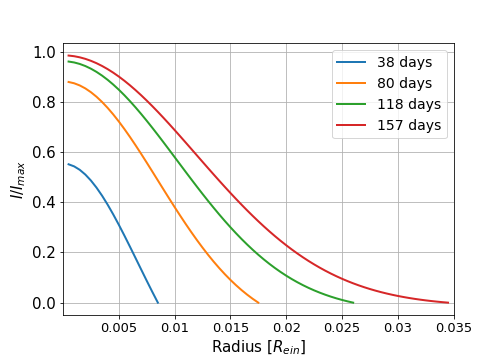
\includegraphics[width=0.8\textwidth]{microlensing/images/profile.png}
	\caption{Нормированный профиль яркости сверхновой в зависимости от радиуса и времени (в системе отсчёта сверхновой) с момента её взрыва ($R_{ein}\approx4.6\cdot10^{14}$ м).}
	\label{fig:profile}
\end{figure}

На Рисунке \ref{fig:example} приведены примеры флуктуации от микролинзирования, рассчитанные по формуле \eqref{eq:deltam}. В одном положении источник при расширении захватывает области сильного усиления, что может заметно повлиять на форму истинной кривой блеска источника (флуктуации $\sim 1$ зв. вел.). В другом положении источник находится в области с практически равномерным усилением и не пересекает каустики; эффект от микролинзирования слабый и примерно постоянный во времени. В каждом положении сверхновая моделировалась диском с плоской засветкой и с гауссовым профилем яркости. Из рисунка можно заключить, что учёт реалистичного распределения яркости сглаживает сильные флуктуации от микролинзирования.

\begin{figure}[H]
    \centering
	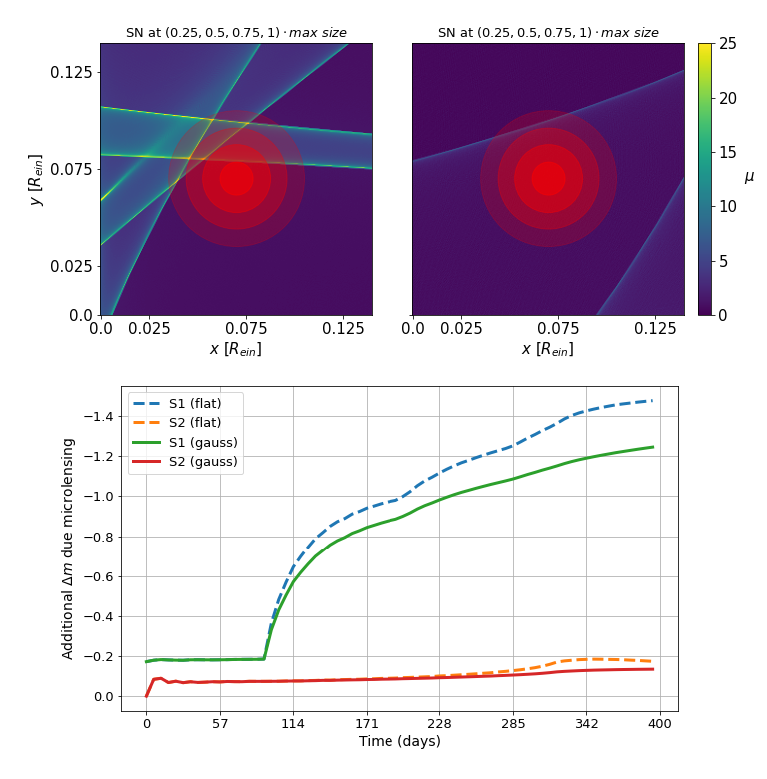
\includegraphics[width=0.99\textwidth]{microlensing/images/caustic.png}
	\caption{\textit{Сверху}: случайные положения сверхновой в изображении S1 (слева) и S2 (справа). \textit{Снизу}: соответствующие этим положениям флуктуации от микролинзирования для источника с плоской засветкой (\textit{flat}) и гауссовым профилем яркости (\textit{gauss}).} 
	\label{fig:example}
\end{figure}

Для статистического анализа микролинзирования был выбран следующий алгоритм. На каждой из карт, изображенных на Рисунке \ref{fig:mymaps}, случайным образом выбираются 50 точек, соответствующих центру расширяющейся сверхновой. Для каждого положения по формуле \eqref{eq:deltam} вычисляются флуктуации микролинзирования и для плоского источника, и для источника с гауссовым профилем яркости. После этого полученные значения прибавляются к кривым блеска SN Refsdal.

%Положения 50 источников на обеих картах и соответствующие им флуктуации приведены на Рисунках \ref{fig:s1} и \ref{fig:s2}.




\section{Влияние микролинзирования на кривые блеска SN Refsdal}
\noindent Идея такая: фиттируем кривую блеска в S1 кривой блеска в S2, сдвигая последнюю по времени и магнитуде (можно в другую сторону, разницы нет). \\ \\
$m_{S1}^{fit} = m_{S2}(t - \Delta t)-\Delta m$ \\

$\log p = -\frac{1}{2} \sum \big( m_{S1} - m_{S1}^{fit} \big)^2$ \rightarrow \max \\ \\

\noindent Подразумевается суммирование по всем точкам на кривой блеска. У меня не учтена модельная погрешность $\sigma_m$ (точнее, она предполагается постоянной). Можно модифицировать функцию правдоподобия следующим образом, но тогда нужно будет заново произвести все расчёты. \\ \\

$\log p = -\frac{1}{2} \sum \frac{( m_{S1} - m_{S1}^{fit} )^2}{\sigma_m^2} + \log \big( 2\pi\sigma_m^2 \big)$ \\ \\

\noindent Из всех кривых $m_{S1}^{fit}$ выбирается та, для которой функция правдоподобия максимальна (это и есть Best fit на рисунке слева), значения $\Delta t$ и $\Delta m$ для неё запоминаются, описанные выше действия повторяются для других реализаций. \\

$\Delta t_{true} = 9.5$ days, 
$\Delta m_{true} = -0.14$ \\
$\Delta t_{best} = -8.6$ days,
$\Delta m_{best} = -0.84$ 


\newpage
\section{Обсуждение}
Для 50 различных случайных положений сверхновой в каждом из двух изображений были рассчитаны флуктуации от микролинзирования для источника с гауссовым профилем яркости. Эти флуктуации, уникальные для каждого изображения, прибавлялись к кривым блеска, на основе чего для каждой из $50 \cdot 50 = 2500$ реализаций были получены распределения значения временной задержки $\Delta t$ и относительного усиления в звёздных величинах $\Delta m$. Гистограммы этих распределений изображены на Рисунке \ref{fig:histograms}.

\begin{figure}[H]
    \centering
	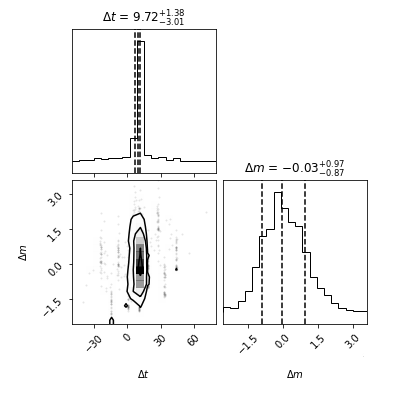
\includegraphics[width=0.6\linewidth]{microlensing/images/histo1.png}
	\caption{Гистограммы, построенные по 2500 значениям временных задержек $\Delta t$ и относительных усилений $\Delta m$.} 
	\label{fig:histograms}
\end{figure}

Гистограммы по всем значениям $\Delta m$ можно трактовать как распределение вероятности усиления (в звездных величинах) вследствие микролинзирования. Гистограммы по значениям $\Delta t$ иллюстрируют возможное влияние микролинзирования на точность оценок временных запаздываний между изображениями, и, как следствие, на точность определения постоянной Хаббла.

На картах, используемых в данной работе, источник чаще попадал в области без каустик, из-за чего для большого количества реализаций микролинзирование вообще никак не сказалось. Это объясняет высокий и узкий пик гистограммы около истинного значения $\Delta t$. Тем не менее, разброс по $\Delta m$ гораздо шире. Это означает, что в реальности затруднительно отделить макроусиление от линзы от микроусиления от отдельных звезд. Из этого можно сделать следующий вывод: в идеальных условиях, когда наблюдения производятся часто и при помощи идеального телескопа, вклад микролинзирования в значения временной задержки и относительного усиления по крайней мере между изображениями S1 и S2 SN Refsdal невелик. Также это может указывать на то, что ошибки величины $\Delta m$ в работах из обзора \cite{treu2016}, возможно, недооценены. %Ошибки в $\Delta t$ из-за микролинзирования сравнимы с ошибками самой величины. 

%Теперь увеличим количество различных положений сверхновой на карте: по 200 на каждой из них, всего 200х200=40000 реализаций. Но теперь только для плоского источника. Гистограмма по 40000 точек не очень сильно отличается от гистограммы для 2500 точек. Возможно, для полноценного статичестического исследования не нужно так много реализаций.


%Открытые вопросы: 
%(а) Будет ли вклад микролинзирования  плоского источника отличаться от гауссового? Для этого нужно знать, какой профиль яркости у SN Refsdal.
%(б) Будут ли ошибки такими же маленькими, если кривая блеска будет наблюдаться после пика или в другом фильтре? В идеале стоит проверить и то, и то, но хочется понимать, корректно ли работает данный алгоритм.
%(в) Есть основания полагать, что dt и dm должны быть скореллированы (например, как в (Kelly et al. 2016). Но нужно ли это учитывать при фиттировании?






\chapter{Заключение}
В данной работе представлен алгоритм извлечения оценки постоянной Хаббла на основе данных по всем 5 изображениям сверхновой SN Refsdal (S1-S4, SX). Исходя из сравнения прогнозов временных задержек и коэффициентов усиления, рассчитанных в различных моделях гравитационного потенциала линзы-галактики и масштабированных таким образом, чтобы они совпадали с наблюдаемыми величинами, вычислено значение постоянной Хаббла, наиболее точно удовлетворяющее и модельным, и наблюдательным данным: $H_0=68.1^{+12.9}_{-10.0}.$  Значение было рассчитано по изображениям SX и S2 сверхновой SN Refsdal. Существенно улучшить оценку величины $H_0$ поможет увеличение числа рассматриваемых гравитационно линзированных систем в целом и более детальная кривая блеска в изображении SX в частности. Полученные результаты также могут послужить независимым тестом различных  моделей распределения масс в линзе-галактике. %Оценка могла бы быть существенно выше, если бы была доступна более детальная кривая блеска для SX.

При анализе гравитационно линзированных сверхновых с наблюдаемыми множественными изображениями одним из важнейших систематических эффектов является микролинзирование звездами галактики-линзы, которое может существенным образом изменять наблюдаемые кривые блеска. Звезды в галактике образуют богатую сеть каустик, что приводит к тому, что наблюдаемые кривые блеска при расширении сверхновых испытывают зависящие от времени усиления/ослабления, уникальные для каждого изображения. Проведено моделирование влияния микролинзирования на кривые блеска сверхновых с коллапсирующим ядром на примере SN Refsdal. Разработан комплекс вычислительных программ, позволяющий учесть реалистичное распределение яркости, а также неточечность источника излучения. На основе проведенного анализа построено распределение вероятности усиления вследствие микролинзирования в звездных величинах и оценено возможное влияние на точность оценок временных запаздываний между изображениями, и, как следствие, на точность определения постоянной Хаббла.

Получена оценка неопределённости, вносимой в определение временных задержек между изображениями S1 и S2 SN Refsdal только микролинзированием в условиях идеального эксперимента. Погрешность составляет 1-3 дня. Таким образом, для определения постоянной Хаббла по гравитационно линзированым сверхновым необходимо использовать системы с временными задержками, составляющими десятки дней. В случае с SN Refsdal это означает, что значение $H_0$ наиболее надежно определяется по паре изображений S2-SX, а анализ изображений S1-S4 позволяет лучше ограничить модель линзы. 

Показано, что даже в условиях идеального эксперимента точность измерения усилений изображений составляет порядка 1 зв.вел. Стоит отметить, что значения макроусиления в моделях линз выводятся, как правило, без учёта микролинзирования. Анализ, проведённый в данной работе, показывает, что, микролинзирование может вносить существенный разброс в определение макроусилений.



%Целью данной работы была оценка возможного вклад микролинзирования при условии проведения идеального эксперимента, в котором гравитационно линзированная система наблюдается практически непрерывно, а ошибки наблюдений сведены к нулю. %Планируется проведение более приближенного к реальности эксперимента, когда учитывается реалистичная частота наблюдений и характеристики настоящих телескопов.
 


\backmatter

\printbib

%\newpage
%\chapter{Приложение}\label{appendix}

\end{document}
